\documentclass[conference]{IEEEtran}
\usepackage{amsmath,amssymb,amsfonts}
\usepackage{graphicx}
\usepackage{textcomp}
\usepackage{xcolor}
\usepackage{hyperref}
\usepackage{booktabs}
\usepackage{algorithm}
\usepackage{algpseudocode}
\usepackage{listings}
\usepackage{multirow}
\usepackage{subcaption}
\usepackage{balance}

\def\BibTeX{{\rm B\kern-.05em{\sc i\kern-.025em b}\kern-.08em
    T\kern-.1667em\lower.7ex\hbox{E}\kern-.125emX}}

\begin{document}

\title{Retrieval Pivot Attacks in Hybrid RAG:\\
Measuring and Mitigating Amplified Leakage from\\
Vector Seeds to Graph Expansion}

\author{
\IEEEauthorblockN{Scott Thornton}
\IEEEauthorblockA{perfecXion.ai \\
scthornton@gmail.com}
}

\maketitle

% ============================================================
\begin{abstract}
Hybrid Retrieval-Augmented Generation (RAG) pipelines that combine
vector similarity search with knowledge graph expansion are increasingly
deployed in enterprise settings for their superior multi-hop reasoning
capabilities. However, this architectural pattern introduces a critical
security vulnerability we term \textbf{Retrieval Pivot Risk (RPR)}:
a semantically retrieved ``seed'' chunk can \emph{pivot} through entity
linking into sensitive graph neighborhoods, yielding data leakage that
is absent in vector-only retrieval.

We formalize RPR and its associated metrics---Amplification Factor (AF),
Pivot Depth (PD), and Leakage@k---and present a taxonomy of four
\textbf{Retrieval Pivot Attacks} that exploit the vector-to-graph
transition with injection budgets as small as 10 chunks. Our evaluation
on a synthetic multi-tenant enterprise corpus (1{,}000 documents,
2{,}785 graph nodes, 15{,}514 edges) with 500 evaluation queries
demonstrates that undefended hybrid pipelines exhibit
$\text{RPR} = 0.95 \pm 0.02$ (95\% CI) and
$\text{AF}(\epsilon) \approx 160\text{--}194\times$ compared to
vector-only retrieval, with all leakage occurring at $\text{PD} = 2$
hops---a structural consequence of the bipartite chunk-entity graph
topology.

We propose and evaluate five layered defenses---per-hop authorization,
edge allowlisting, budgeted traversal, trust-weighted expansion, and
merge-time policy filtering---showing that per-hop authorization alone
eliminates all measured leakage ($\text{RPR} \to 0.0$) across both
benign and adversarial queries, including all four attack variants, while
retaining 50\% of graph-expanded context. The full defense stack further
reduces context noise by 82\%, reaching 19--20 items from a baseline
of 110.
\end{abstract}

\begin{IEEEkeywords}
retrieval-augmented generation, knowledge graphs, adversarial machine
learning, hybrid RAG, graph security, data exfiltration, access control
\end{IEEEkeywords}

% ============================================================
\section{Introduction}
\label{sec:introduction}

Enterprise adoption of Retrieval-Augmented Generation (RAG) has
accelerated rapidly: 30--60\% of enterprise AI use cases now rely on
RAG architectures~\cite{saferag2025}, and the vector database market
reached \$1.73 billion in 2024~\cite{pineconerac2024}. To improve
multi-hop reasoning over complex organizational knowledge,
practitioners increasingly deploy \emph{hybrid} RAG pipelines that
combine vector similarity search with knowledge graph
expansion~\cite{hybridrag2024, microsoftgraphrag2024}. These systems
retrieve an initial set of text chunks via embedding similarity, then
\emph{pivot} through entity mentions into a knowledge graph to gather
structurally related context before passing the assembled results to a
large language model (LLM).

This pivot mechanism---the vector-to-graph transition---introduces a
security boundary that no prior work has studied. Consider an analyst
at an engineering firm who queries a hybrid RAG system about Kubernetes
cluster configurations. Vector retrieval returns authorized
engineering documents. But those documents mention shared entities
(``CloudCorp,'' ``auth-service'') that also appear in the knowledge
graph connected to confidential HR salary records, restricted security
credentials, and financial audit data belonging to other tenants. A
2-hop graph expansion from the authorized seed chunks traverses
through these shared entities into unauthorized neighborhoods,
silently injecting sensitive cross-tenant data into the analyst's
context window.

Prior work has studied vector-side poisoning in
isolation~\cite{zou2025poisonedrag, corruptrag2025, ctrlrag2025} and
graph-side attacks independently~\cite{gragpoison2026, fewwords2025,
ragsafety2025}. PoisonedRAG achieves 90\% attack success rate by
injecting 5 malicious texts into vector stores~\cite{zou2025poisonedrag}.
GRAGPoison demonstrates 98\% success via relation-centric poisoning
within GraphRAG~\cite{gragpoison2026}. Yet neither addresses what
happens at the \emph{boundary} between these stores---the point where
vector retrieval results become graph traversal seeds. The
OWASP LLM Top 10 (2025) introduced LLM08 (Vector and Embedding
Weaknesses) but does not address graph
components~\cite{owasptop10llm2025}. MITRE ATLAS treats RAG as a
monolithic system~\cite{mitreatlas2025}. The SoK on RAG privacy
explicitly identifies hybrid RAG security as an open
problem~\cite{sokprivacy2026}.

This paper makes three contributions:

\begin{enumerate}
\item \textbf{Formalization.} We define Retrieval Pivot Risk (RPR)
  and companion metrics---Amplification Factor (AF, AF($\epsilon$)),
  Pivot Depth (PD), Leakage@k, severity-weighted leakage, and
  $\Delta$Leakage---that quantify the security impact of the
  vector-to-graph transition (\S\ref{sec:metrics}).

\item \textbf{Attack taxonomy.} We present four Retrieval Pivot
  Attacks---Seed Steering (A1), Entity Anchor Injection (A2),
  Neighborhood Flooding (A3), and Bridge Node Attack
  (A4)---that exploit the pivot boundary with injection budgets of
  10--20 chunks. We evaluate all four attacks against multiple
  defense configurations (\S\ref{sec:attacks}).

\item \textbf{Defense suite and analysis.} We design and evaluate
  five layered defenses (D1--D5) that operate across the
  vector-to-graph boundary. Our analysis reveals that the critical
  defense placement is \emph{at the graph expansion boundary}: per-hop
  authorization (D1) eliminates all measured leakage while the
  remaining defenses (D2--D5) serve as utility optimizers and
  defense-in-depth layers (\S\ref{sec:mitigations}). We further
  characterize the \emph{amplification mechanics} of the pivot---why
  graph expansion transforms authorized vector results into
  unauthorized graph traversals---and identify the total node budget
  as the primary leakage-controlling parameter through a 27-configuration
  traversal sweep (\S\ref{sec:results}).
\end{enumerate}

Our key finding is both surprising and practically significant:
\emph{a single defense---per-hop authorization that re-checks tenant
and sensitivity labels at each graph expansion step---completely
eliminates retrieval pivot leakage across 500 evaluation queries,
all four attack variants, and metadata mislabel rates up to 5\%.}
This defense is simple to implement, requires no model changes, and
adds negligible latency ($<$1ms overhead).

The complete codebase, data generators, attack implementations,
defense suite, and experimental results are available at
\url{https://github.com/scthornton/hybrid-rag-pivot-attacks}.

% ============================================================
\section{Background}
\label{sec:background}

\subsection{Vector Retrieval in RAG}

Standard RAG systems encode documents as dense vector embeddings using
models such as all-MiniLM-L6-v2~\cite{corpuspoisoning2023} and
retrieve the top-$k$ chunks by cosine similarity to the query
embedding. In multi-tenant deployments, vector stores apply metadata
prefilters (e.g., tenant ID) before similarity search, ensuring that
retrieval respects organizational boundaries. This prefiltering makes
vector-only RAG robust against cross-tenant leakage: our experiments
confirm $\text{RPR} = 0.0$ for vector-only pipelines across all 500
evaluation queries (\S\ref{sec:results}).

\subsection{Knowledge Graph RAG}

GraphRAG~\cite{microsoftgraphrag2024} and related approaches
construct knowledge graphs from document corpora via named entity
recognition (NER) and relation extraction, then leverage graph
structure for multi-hop reasoning. Systems like
AgCyRAG~\cite{agcyrag2025} use LLM-driven graph traversal for
complex queries. Graph-based retrieval provides superior
comprehensiveness on multi-hop queries---86\% versus 57\% for vector
RAG~\cite{hybridrag2024}---but introduces graph-specific attack
surfaces: GRAGPoison~\cite{gragpoison2026} achieves 98\% attack
success through relation-centric poisoning, and TKPA~\cite{fewwords2025}
drops QA accuracy from 95\% to 50\% by modifying just 0.06\% of
corpus text.

\subsection{Hybrid RAG and the Pivot Boundary}

Hybrid RAG combines both retrieval modalities in a pipeline:

\begin{enumerate}
\item \textbf{Vector retrieval:} Query embedding $\rightarrow$ cosine
  similarity $\rightarrow$ top-$k$ seed chunks $S(q)$.
\item \textbf{Entity linking:} Extract named entities from $S(q)$ via
  NER; map entity mentions to knowledge graph node IDs.
\item \textbf{Graph expansion:} BFS/DFS traversal from linked entity
  nodes to depth $d$, gathering structurally related nodes.
\item \textbf{Context merge:} Combine vector-retrieved chunks with
  graph-expanded context for LLM generation.
\end{enumerate}

We define the \textbf{pivot boundary} as the transition between steps
1--2 and steps 3--4: the point where vector retrieval results become
graph traversal seeds. This boundary is the attack surface we study.
Vector-side prefilters operate \emph{before} the pivot; graph
expansion operates \emph{after} it. If graph expansion does not
independently enforce access controls, any entity mentioned in an
authorized seed chunk becomes an uncontrolled entry point into the
knowledge graph.

% ============================================================
\section{Threat Model}
\label{sec:threat_model}

\subsection{System Model}

We consider a multi-tenant enterprise hybrid RAG system with the
following components:

\begin{itemize}
\item A \textbf{vector store} (ChromaDB) containing document chunk
  embeddings with tenant and sensitivity metadata.
\item A \textbf{knowledge graph} (Neo4j) containing entity nodes,
  chunk nodes, and typed edges (MENTIONS, DEPENDS\_ON, BELONGS\_TO,
  RELATED\_TO) extracted from the document corpus.
\item An \textbf{entity linker} that maps NER-extracted entities from
  vector-retrieved chunks to graph node IDs.
\item A \textbf{graph expander} that performs BFS traversal from
  linked entities to depth $d$ (default $d=2$), implemented via
  Neo4j's \texttt{apoc.path.spanningTree} for hop-distance tracking.
\item Four organizational \textbf{tenants} with distinct data
  ownership boundaries.
\item Four \textbf{sensitivity tiers}: PUBLIC ($\approx$40\% of
  corpus), INTERNAL (30\%), CONFIDENTIAL (20\%), RESTRICTED (10\%).
\end{itemize}

\subsection{Attacker Capabilities}

We consider two attacker models:

\textbf{Injection attacker.} The attacker holds a legitimate account
in one tenant (\texttt{acme\_engineering}) and can inject documents
into the shared corpus through standard channels---wiki edits, ticket
updates, shared document repositories. Injected documents undergo
normal ingestion: chunking, NER-based entity extraction, embedding,
and indexing into both vector and graph stores. The attacker's
injection budget is modest: 10--20 chunks, consistent with the budgets
shown effective in prior work~\cite{zou2025poisonedrag,
corruptrag2025}.

\textbf{No-injection attacker.} The attacker holds a legitimate
account and crafts queries that mention bridge entities (shared
infrastructure names, vendor references, cross-team personnel) to
maximize pivot probability through naturally occurring cross-tenant
entity connections. This attacker requires \emph{zero document
injection}---the organic structure of the multi-tenant knowledge graph
provides the pivot paths. Our evaluation shows that this attacker
model achieves $\text{RPR} = 0.95$ through benign queries alone
(\S\ref{sec:results}), demonstrating that the vulnerability is
\emph{structural} rather than injection-dependent.

\subsection{Attacker Goals}

\begin{itemize}
\item \textbf{G1: Cross-tenant access.} Cause the retrieval context
  for a query in the attacker's tenant to include chunks or entities
  belonging to other tenants.
\item \textbf{G2: Sensitivity escalation.} Cause an INTERNAL-clearance
  user's context to include CONFIDENTIAL or RESTRICTED items.
\item \textbf{G3: Amplified leakage.} Achieve leakage in the hybrid
  pipeline that exceeds what is possible with vector-only retrieval
  (i.e., $\text{AF} > 1$).
\end{itemize}

\subsection{Adaptive Attacker Considerations}

An adaptive attacker aware of D1 (per-hop authorization) might
attempt to bypass it through: (a) \textbf{metadata spoofing}---forging
tenant or sensitivity labels during document injection, or
(b) \textbf{same-tenant escalation}---crafting documents within the
attacker's own tenant that link to higher-sensitivity content within
the same tenant boundary. D1 is robust against (a) if and only if the
ingestion pipeline enforces metadata integrity (the metadata
is assigned by the system, not the uploader). We evaluate D1's
robustness under metadata corruption in \S\ref{sec:mislabel} and
discuss mitigation strategies in \S\ref{sec:metadata-integrity}.
Same-tenant escalation (b) targets \emph{sensitivity} boundaries
rather than \emph{tenant} boundaries and requires the attacker to
already have write access to the target tenant's corpus.

\subsection{Scope}

We focus exclusively on the \emph{retrieval layer}: measuring what
unauthorized content enters the LLM's context window. We do not
evaluate LLM generation quality, jailbreaking, or prompt injection.
The attacker does not have direct database access, cannot modify model
weights, and cannot alter the pipeline configuration. We omit a
graph-only baseline (P2) because graph-only RAG without vector
seeding is a fundamentally different retrieval paradigm that does not
involve the pivot boundary we study; its security properties are
addressed by prior work on GraphRAG
attacks~\cite{gragpoison2026, fewwords2025}.

% ============================================================
\section{Retrieval Pivot Attacks}
\label{sec:attacks}

We define four attacks that exploit the pivot boundary with
increasing structural sophistication. Each attack operates within the
threat model of \S\ref{sec:threat_model}: the attacker injects a
small number of crafted documents that undergo standard ingestion.

\subsection{A1: Seed Steering}

\textbf{Objective.} Maximize the probability that attacker-crafted
chunks are retrieved by target queries while embedding entity mentions
that link to sensitive graph neighborhoods.

\textbf{Mechanism.} The attacker estimates the query centroid for
target query families (e.g., ``infrastructure monitoring'') and crafts
10 chunks with high semantic overlap to this centroid. Each chunk
embeds 2 pivot entities---entities that are within 1--2 hops of
sensitive nodes in the knowledge graph (e.g., \texttt{k8s-prod-cluster},
\texttt{auth-service}). Chunks are labeled PUBLIC with low provenance
scores (0.3) to bypass any trust-based filtering. When retrieved,
entity linking maps the embedded entity mentions to graph nodes,
seeding expansion into sensitive neighborhoods.

\textbf{Entry point.} Vector retrieval (cosine similarity).\\
\textbf{Pivot mechanism.} Entity linking from retrieved chunk to
graph node.

\subsection{A2: Entity Anchor Injection}

\textbf{Objective.} Force entity linking to create dense connections
between injected chunks and sensitive graph neighborhoods.

\textbf{Mechanism.} The attacker identifies anchor entities adjacent
to sensitive nodes (e.g., entities 1 hop from restricted credentials)
and crafts chunks with dense entity mentions: 3+ mentions of the
primary target entity per chunk, plus 2 related entities. NER
extraction creates MENTIONS edges from each chunk to the target
entities. Any query that retrieves one of these chunks---even
incidentally---triggers graph expansion toward the sensitive area.

\textbf{Entry point.} Entity extraction during ingestion.\\
\textbf{Pivot mechanism.} MENTIONS edges from chunk to target entity
nodes.

\subsection{A3: Neighborhood Flooding}

\textbf{Objective.} Inflate the local density around a target entity
to increase the volume of sensitive content reachable through BFS
expansion.

\textbf{Mechanism.} The attacker injects 20 chunks, each mentioning
a high-value target entity near a sensitive subgraph. Each chunk also
mentions a different neighbor entity, creating a dense web of edges.
The result is a ``graph gravity well'': the target entity accumulates
many more edges than the graph average, causing BFS expansion to
gather a larger neighborhood when traversing through this entity.
Note that our pipeline uses uniform BFS traversal (not degree-weighted
or PageRank-based expansion), so the flooding increases reachable
volume rather than biasing traversal order.

\textbf{Entry point.} Graph topology manipulation via ingestion.\\
\textbf{Pivot mechanism.} Inflated local density increases BFS
expansion volume.

\subsection{A4: Bridge Node Attack}

\textbf{Objective.} Create artificial cross-tenant edges that enable
graph traversal from the attacker's tenant into a target tenant.

\textbf{Mechanism.} The attacker crafts 15 chunks that co-mention
entities from both the attacker's tenant and the target tenant within
the same document. NER extraction creates entity nodes on both sides
of the tenant boundary, and relation extraction creates RELATED\_TO
edges between them. After ingestion, BFS expansion from the
attacker's authorized subgraph can traverse these artificial bridge
edges into the target tenant's data.

\textbf{Entry point.} Cross-tenant entity co-mention.\\
\textbf{Pivot mechanism.} Artificial RELATED\_TO edges spanning tenant
boundaries.

\medskip

Algorithm~\ref{alg:pivot_attack} formalizes the general pivot attack
framework.

\begin{algorithm}[t]
\caption{General Retrieval Pivot Attack}
\label{alg:pivot_attack}
\begin{algorithmic}[1]
\Require Target query family $\mathcal{Q}_T$, injection budget $B$,
  pivot entities $E_p$, target neighborhood $N_T$
\Ensure Injected chunks $C_\text{atk}$
\For{$i = 1$ to $B$}
  \State $c_i \leftarrow$ \Call{CraftChunk}{$\mathcal{Q}_T$, $E_p$}
  \Comment{High similarity to $\mathcal{Q}_T$}
  \State $c_i.\text{entities} \leftarrow$ \Call{EmbedEntities}{$E_p$, $N_T$}
  \Comment{Mentions near $N_T$}
  \State $c_i.\text{sensitivity} \leftarrow$ PUBLIC
  \State $c_i.\text{provenance} \leftarrow 0.3$
  \State $C_\text{atk} \leftarrow C_\text{atk} \cup \{c_i\}$
\EndFor
\State \Call{Ingest}{$C_\text{atk}$}
\Comment{Standard pipeline: chunk, NER, embed, index}
\State \Return $C_\text{atk}$
\end{algorithmic}
\end{algorithm}

% ============================================================
\section{Metrics}
\label{sec:metrics}

We introduce metrics to quantify retrieval pivot risk. Let $q$
denote a query, $u$ a user with tenant $t_u$ and clearance level
$\ell_u$, $S_k(q)$ the top-$k$ context set, and
$\text{Sensitive}(x, u)$ a predicate that is true when item $x$ has
sensitivity $> \ell_u$ or tenant $\neq t_u$. Let
$\text{Seeds}(q) \subseteq S_k(q)$ denote the set of entity nodes
that are linked from vector-retrieved chunks via NER extraction---these
are the graph entry points that initiate BFS expansion.

\subsection{Retrieval Pivot Risk (RPR)}

RPR measures the probability that a query's retrieval context contains
any unauthorized item:

\begin{equation}
\text{RPR}(u) = \Pr_{q \sim \mathcal{Q}}\left[\exists x \in S_k(q):
  \text{Sensitive}(x, u)\right]
\label{eq:rpr}
\end{equation}

\noindent RPR is operationalized as the fraction of evaluation queries
whose context contains at least one sensitive item. We report RPR
with 95\% bootstrap confidence intervals (10{,}000 resamples).

\subsection{Leakage@k}

Leakage@k counts the number of unauthorized items in the context:

\begin{equation}
\text{Leakage@k}(q, u) = \left|\{x \in S_k(q) :
  \text{Sensitive}(x, u)\}\right|
\label{eq:leakage}
\end{equation}

\noindent While RPR captures \emph{whether} leakage occurs,
Leakage@k captures its \emph{severity}. A context with 1 leaked item
and one with 20 both yield $\text{RPR} = 1$, but their Leakage@k
values differ by $20\times$.

\subsection{Severity-Weighted Leakage}

Not all leakage is equally harmful. A PUBLIC-clearance user receiving
INTERNAL content is a lesser violation than receiving RESTRICTED
content. We define severity-weighted leakage as:

\begin{equation}
\text{SWL}(q, u) = \sum_{x \in S_k(q),\; \text{Sensitive}(x,u)}
  \left(\ell_x - \ell_u\right)
\label{eq:swl}
\end{equation}

\noindent where $\ell_x$ is the sensitivity level of item $x$
(PUBLIC=0, INTERNAL=1, CONFIDENTIAL=2, RESTRICTED=3) and $\ell_u$ is
the user's clearance level. Each leaked item contributes weight
proportional to the sensitivity gap it crosses. In our experiments,
the INTERNAL-clearance evaluation user observing RESTRICTED items
produces weight 2 per item, while CONFIDENTIAL items produce weight 1.

\subsection{Amplification Factor}

AF quantifies the leakage increase that hybrid retrieval introduces
compared to vector-only retrieval:

\begin{equation}
\text{AF} = \frac{\mathbb{E}[\text{Leakage@k}]_{\text{hybrid}}}%
  {\mathbb{E}[\text{Leakage@k}]_{\text{vector}}}
\label{eq:af}
\end{equation}

\noindent When the vector baseline produces zero leakage (which our
experiments confirm), $\text{AF} = \infty$ for any nonzero hybrid
leakage. To provide a finite, plottable alternative, we also report
$\text{AF}(\epsilon)$:

\begin{equation}
\text{AF}(\epsilon) = \frac{\mathbb{E}[\text{Leakage@k}]_{\text{hybrid}}}%
  {\max(\mathbb{E}[\text{Leakage@k}]_{\text{vector}},\; \epsilon)}
\label{eq:af_eps}
\end{equation}

\noindent with $\epsilon = 0.1$, alongside the absolute difference
$\Delta\text{Leakage} = \mathbb{E}[\text{Leakage@k}]_{\text{hybrid}}
- \mathbb{E}[\text{Leakage@k}]_{\text{vector}}$.

\subsection{Pivot Depth (PD)}

PD measures the minimum graph distance from a seed node to the first
sensitive node reached during expansion:

\begin{equation}
\text{PD}(q) = \min\{d(s, x) : s \in \text{Seeds}(q),\;
  x \in S_k(q),\; \text{Sensitive}(x, u)\}
\label{eq:pd}
\end{equation}

\noindent where $d(s, x)$ is the shortest-path distance in the
knowledge graph from seed $s$ to node $x$, computed via
\texttt{apoc.path.spanningTree} which yields paths with explicit hop
counts. We report PD as a distribution (min, median, max) across
queries that exhibit leakage, rather than a single summary statistic.

% ============================================================
\section{Experimental Setup}
\label{sec:setup}

\subsection{Synthetic Enterprise Corpus}

We generate a multi-tenant enterprise corpus of 1{,}000 documents
across four organizational tenants: \texttt{acme\_engineering},
\texttt{globex\_finance}, \texttt{initech\_hr}, and
\texttt{umbrella\_security}. Documents are produced by 12
domain-specific generators (3 per tenant) that embed realistic entity
mentions---system names, personnel, projects, compliance
standards---using curated entity pools.

Sensitivity tiers follow a realistic distribution: PUBLIC (40\%),
INTERNAL (30\%), CONFIDENTIAL (20\%), and RESTRICTED (10\%). Each
document includes ground-truth entity annotations and sensitivity
labels.

\textbf{Bridge entities.} We inject 15 bridge entities across 5
categories (shared vendors, shared infrastructure, shared personnel,
shared compliance standards, and shared projects) that naturally
appear in documents across multiple tenants. For example,
``CloudCorp'' appears in both engineering and finance documents,
and ``auth-service'' appears in both engineering and security
documents. After NER-based entity extraction, the knowledge graph
contains 40 naturally shared entities across tenant boundaries---not
through adversarial injection, but through legitimate cross-team
references that any multi-tenant organization would exhibit.

\subsection{Knowledge Graph Construction}

Documents undergo chunking (512-token windows, 50-token overlap),
spaCy NER extraction (\texttt{en\_core\_web\_sm}), two-pass
relation extraction (ground-truth relation resolution followed by
pattern-based extraction across 5 typed relations: DEPENDS\_ON,
OWNED\_BY, BELONGS\_TO, CONTAINS, DERIVED\_FROM, plus RELATED\_TO
fallback), and embedding via all-MiniLM-L6-v2 (384 dimensions). The
resulting graph contains 2{,}785 nodes (785 entity nodes + 2{,}000
chunk nodes) and 15{,}514 edges.

\subsection{Pipeline Variants}

We evaluate 7 pipeline configurations (Table~\ref{tab:variants}):

\begin{table}[t]
\centering
\caption{Pipeline variants and their defense configurations.}
\label{tab:variants}
\small
\begin{tabular}{l|l|l}
\toprule
\textbf{ID} & \textbf{Pipeline} & \textbf{Defenses} \\
\midrule
P1 & Vector-only & Tenant prefilter \\
P3 & Hybrid baseline & None \\
P4 & Hybrid + D1 & Per-hop authz \\
P5 & Hybrid + D1,D2 & + Edge allowlist \\
P6 & Hybrid + D1--D3 & + Budgeted traversal \\
P7 & Hybrid + D1--D4 & + Trust weighting \\
P8 & Hybrid + D1--D5 & + Merge filter \\
\bottomrule
\end{tabular}
\end{table}

\noindent We omit a graph-only baseline (P2) because graph-only
retrieval without vector seeding is a fundamentally different
paradigm that does not involve the pivot boundary under study. Its
security properties are addressed by prior work on GraphRAG
attacks~\cite{gragpoison2026, fewwords2025}.

\subsection{Evaluation Protocol}

We evaluate each pipeline on 500 template-generated queries: 350
benign queries (standard domain questions stratified across 4 tenants
and 3 clearance levels) and 150 adversarial queries (queries that
mention bridge entities or target cross-tenant pivot paths, stratified
across attack types A1--A4). The evaluation user belongs to
\texttt{acme\_engineering} with INTERNAL clearance. For each query,
we measure RPR, Leakage@k, severity-weighted leakage, AF($\epsilon$),
$\Delta$Leakage, PD distribution, latency, and context size. All RPR
and Leakage@k values are reported with 95\% bootstrap confidence
intervals (10{,}000 resamples, seed 42). Graph expansion uses
\texttt{apoc.path.spanningTree} for BFS with hop-distance tracking:
each expanded node records its minimum distance from the nearest seed,
enabling precise PD measurement.

\subsection{Attack Evaluation}

We evaluate all four attacks (A1--A4) against the undefended hybrid
pipeline (P3) and three defense configurations (P4, P6, P8). For each
attack, payloads are injected into a clean corpus, and 10 adversarial
queries are executed against each pipeline variant. After each attack
evaluation, the graph is rebuilt from the clean corpus to prevent
cross-contamination between attack experiments.

% ============================================================
\section{Results}
\label{sec:results}

\subsection{Hybrid RAG Amplifies Leakage}

Table~\ref{tab:defense-ablation} presents security metrics across all
pipeline variants. The central finding is stark: \textbf{the
undefended hybrid pipeline (P3) leaks massively while the vector-only
baseline (P1) leaks nothing.}

P1 achieves $\text{RPR} = 0.0$ on both query sets---the vector
store's tenant prefilter prevents any cross-tenant or
sensitivity-escalated content from reaching the context. In contrast,
P3 achieves $\text{RPR} = 0.954$ [95\% CI: 0.931, 0.974] on 350
benign queries (334 of 350 queries produce leakage) and
$\text{RPR} = 0.947$ [0.907, 0.980] on 150 adversarial queries (142
of 150 queries leak). Mean Leakage@k reaches 16.0 items for benign
queries and 19.4 for adversarial queries---meaning that roughly
15--18\% of the 110-item context consists of unauthorized content.
Severity-weighted leakage averages 22.9 (benign) and 26.4
(adversarial), indicating that leaked items skew toward higher
sensitivity tiers.

\begin{table*}[t]
\centering
\caption{Defense ablation: security metrics across pipeline variants
  (500 queries: 350 benign + 150 adversarial). RPR = Retrieval Pivot
  Risk with 95\% bootstrap CI, Leak = mean Leakage@k, SWL =
  severity-weighted leakage, PD = Pivot Depth (hops), Ctx = mean
  context size. ``--'' indicates no leakage occurred (PD undefined).}
\label{tab:defense-ablation}
\small
\begin{tabular}{l|ccccc|ccccc}
\toprule
 & \multicolumn{5}{c|}{\textbf{Benign Queries ($n=350$)}} &
   \multicolumn{5}{c}{\textbf{Adversarial Queries ($n=150$)}} \\
\textbf{Variant} & RPR [CI] & Leak & SWL & PD & Ctx &
  RPR [CI] & Leak & SWL & PD & Ctx \\
\midrule
P1 (Vector) & 0.000 & 0.0 & 0.0 & -- & 10 &
  0.000 & 0.0 & 0.0 & -- & 10 \\
P3 (Hybrid) & .954 [.931,.974] & 16.0 & 22.9 & 2.0 & 110 &
  .947 [.907,.980] & 19.4 & 26.4 & 2.0 & 110 \\
P4 (+D1) & 0.000 & 0.0 & 0.0 & -- & 56 &
  0.000 & 0.0 & 0.0 & -- & 50 \\
P5 (+D1,D2) & 0.000 & 0.0 & 0.0 & -- & 57 &
  0.000 & 0.0 & 0.0 & -- & 51 \\
P6 (+D1--D3) & 0.000 & 0.0 & 0.0 & -- & 29 &
  0.000 & 0.0 & 0.0 & -- & 28 \\
P7 (+D1--D4) & 0.000 & 0.0 & 0.0 & -- & 28 &
  0.000 & 0.0 & 0.0 & -- & 24 \\
P8 (All) & 0.000 & 0.0 & 0.0 & -- & 20 &
  0.000 & 0.0 & 0.0 & -- & 20 \\
\bottomrule
\end{tabular}
\end{table*}

Because the vector baseline produces zero leakage, the classical
Amplification Factor is formally infinite: $\text{AF} = \infty$. Using
the regularized metric, $\text{AF}(\epsilon{=}0.1) = 159.9$ for benign
queries and $193.8$ for adversarial queries. The absolute difference
$\Delta\text{Leakage} = 16.0$ (benign) and $19.4$ (adversarial).
These complementary metrics confirm the same finding: graph expansion
introduces leakage that is \emph{entirely absent} in vector-only
retrieval. The hybrid architecture does not merely amplify existing
risk---it creates risk from nothing.

Figure~\ref{fig:rpr} shows RPR with bootstrap confidence intervals
across pipeline variants.

\begin{figure}[t]
\centering
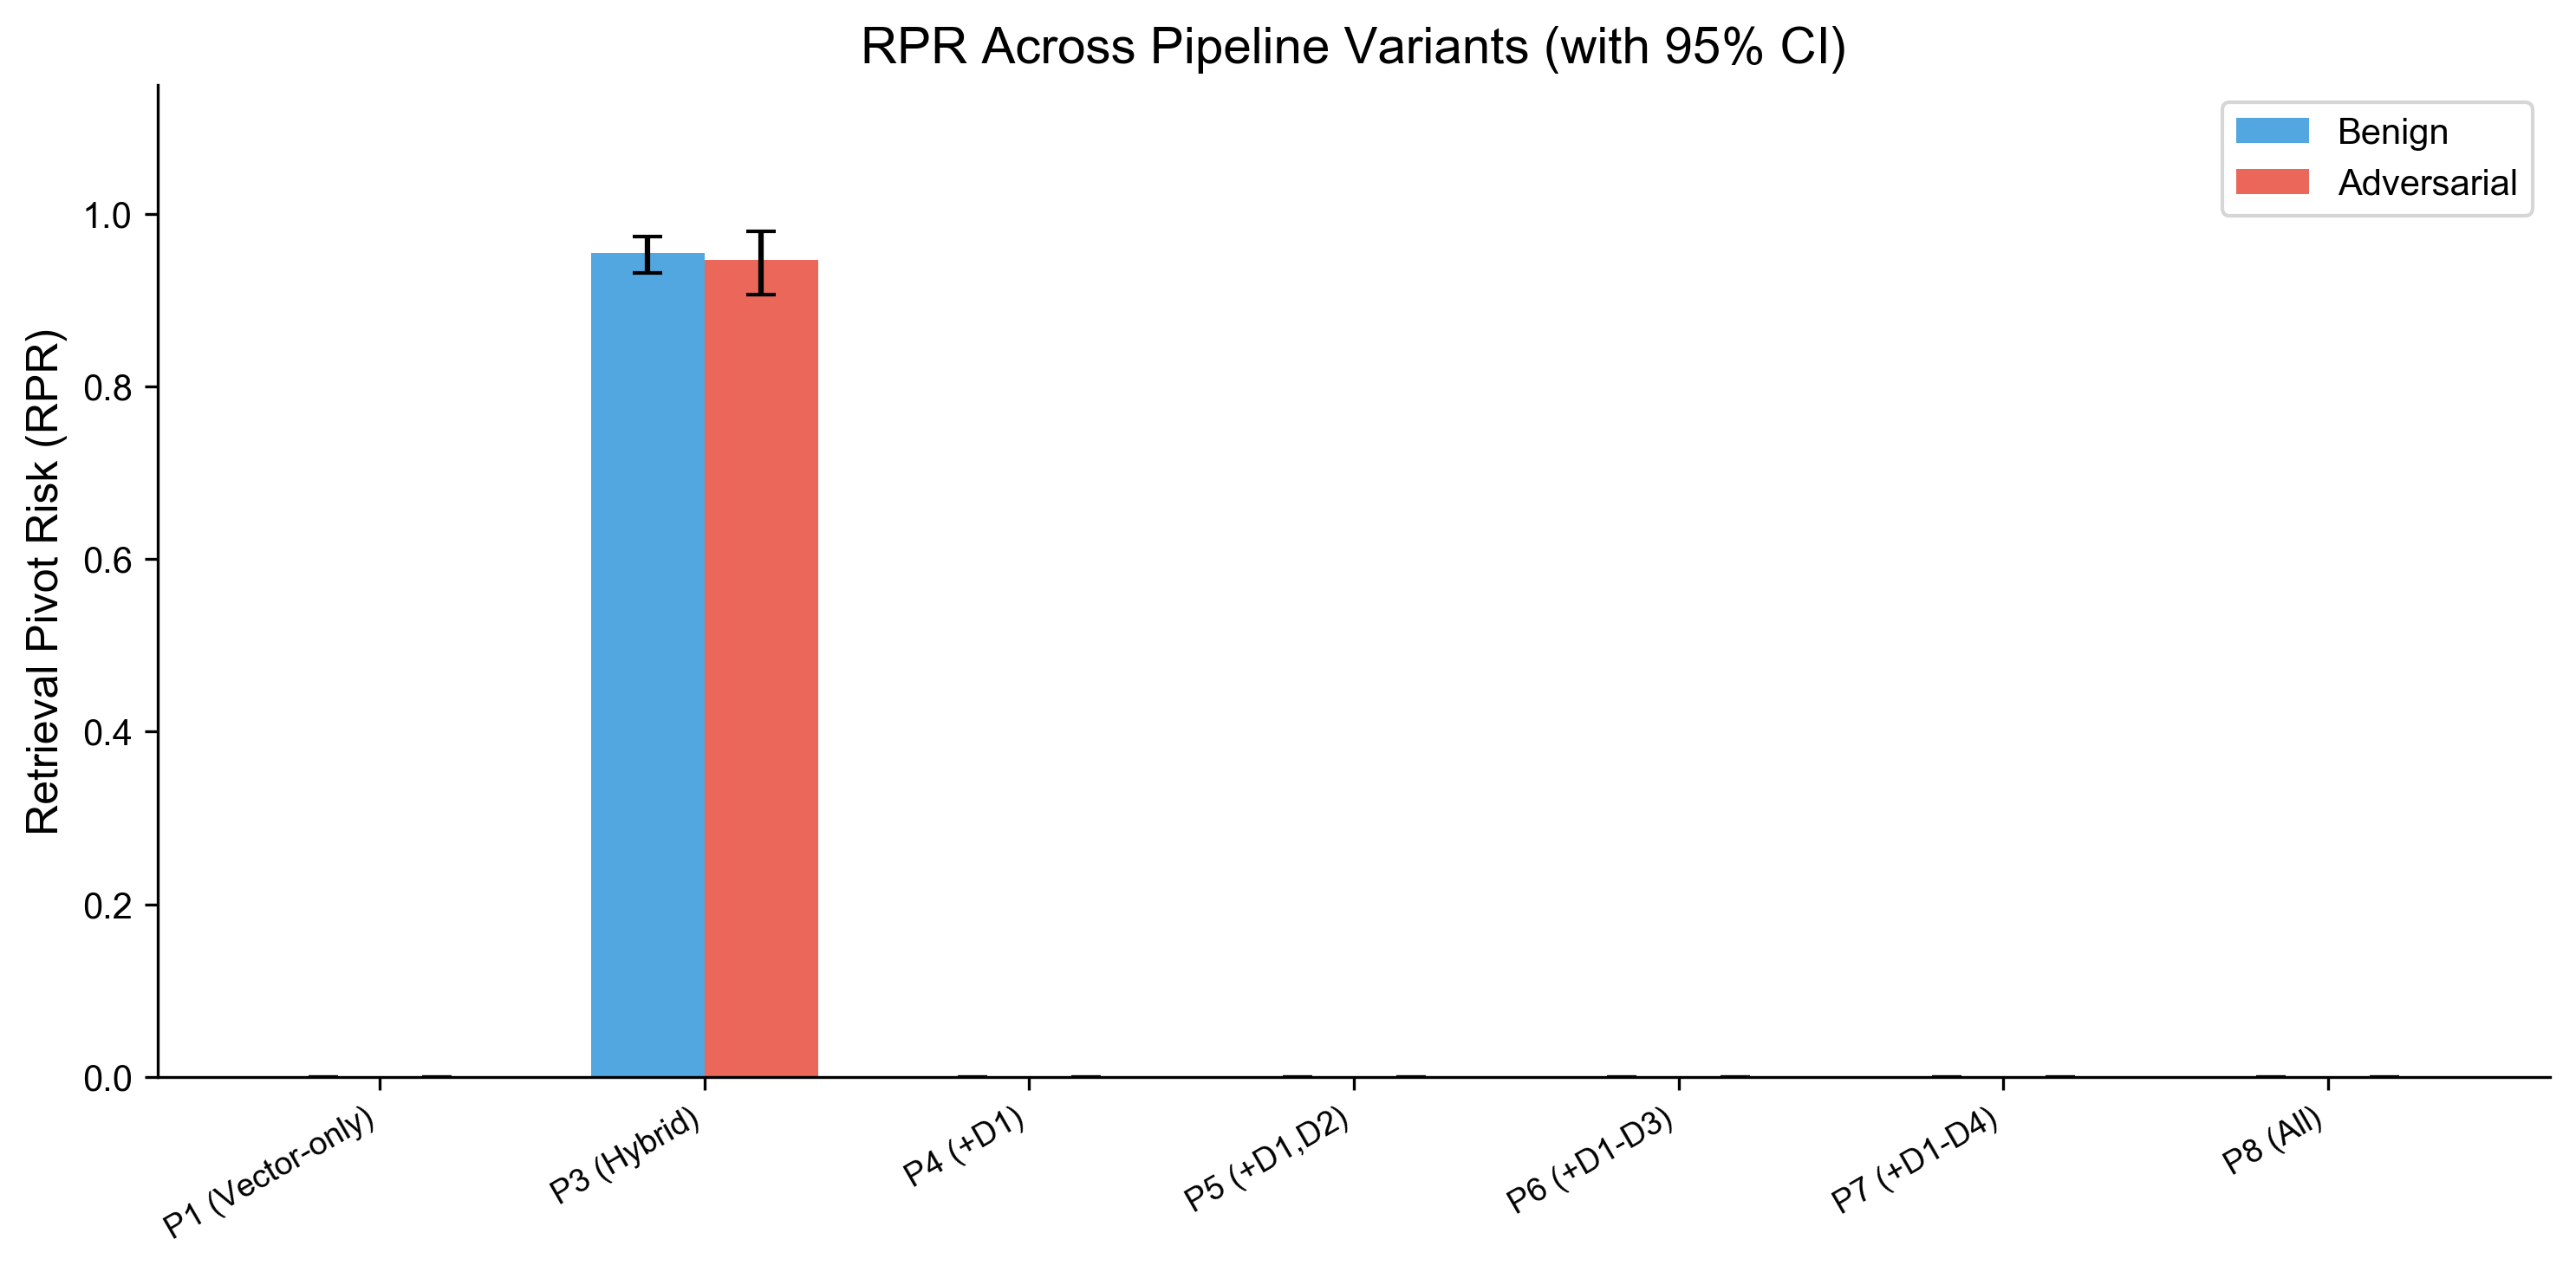
\includegraphics[width=\columnwidth]{figures/rpr_with_ci.png}
\caption{Retrieval Pivot Risk with 95\% bootstrap CIs across pipeline
  variants. P3 (undefended hybrid) shows
  $\text{RPR} \approx 0.95$. All defended variants (P4--P8) achieve
  $\text{RPR} = 0.0$.}
\label{fig:rpr}
\end{figure}

\subsection{The PD = 2 Structural Signature}

All leakage in P3 occurs at exactly $\text{PD} = 2$ hops: the PD
distribution is $(\min=2, \text{median}=2, \max=2)$ across all 476
leaking queries. This uniformity is not coincidental---it is a
structural consequence of the bipartite chunk-entity graph topology in
our construction. The pivot path is:

\begin{enumerate}
\item \textbf{Hop 0}: Authorized seed chunk (retrieved by vector
  similarity, passes tenant prefilter).
\item \textbf{Hop 1}: Shared entity node (linked via NER from seed
  chunk text; entity nodes carry no tenant ownership).
\item \textbf{Hop 2}: Unauthorized chunk (connected to the shared
  entity via MENTIONS edge; belongs to a different tenant or higher
  sensitivity tier).
\end{enumerate}

This 2-hop pattern is inherent to any hybrid RAG system that
constructs a bipartite graph between chunks and entities with
expansion depth $d \geq 2$: the entity-linking step creates a
structural bridge between vector-retrieved content and graph-stored
content. The PD=2 finding is \emph{structural in our bipartite
construction}---knowledge graphs with richer entity-to-entity
relationships (e.g., ontological hierarchies, multi-hop inference
chains) may exhibit leakage at deeper pivot depths. We discuss
how PD varies with traversal parameters in
\S\ref{sec:traversal-sweep}.

\subsection{Organic Leakage: No Injection Required}
\label{sec:organic}

A critical observation from our 350 benign queries is that
$\text{RPR} = 0.954$ \emph{without any adversarial injection}. The
40 naturally shared entities across tenant boundaries---shared
infrastructure, vendors, personnel, compliance standards, and
projects---provide sufficient pivot paths for massive leakage through
ordinary queries. In our corpus, 334 of 350 benign queries (95.4\%)
trigger cross-tenant leakage through organic entity connections. This
means the vulnerability is \emph{structural}: it exists in any
multi-tenant hybrid RAG deployment where tenants share real-world
entities, regardless of whether an attacker injects content.

\textbf{Bridge category analysis.} To understand which types of
shared entities drive leakage, we analyze the hop-1 pivot nodes in
each leaking query's traversal path and classify them against the 5
bridge entity categories (Table~\ref{tab:organic-leakage}).

\begin{table}[t]
\centering
\caption{Organic leakage by bridge entity category under P3 (no
  injection). Queries = leaking queries with that bridge type at
  hop 1. Leak = attributed leaked items.}
\label{tab:organic-leakage}
\small
\begin{tabular}{l|rr|rr}
\toprule
\textbf{Bridge Category} & \multicolumn{2}{c|}{\textbf{Benign}} &
  \multicolumn{2}{c}{\textbf{Adversarial}} \\
 & Queries & Leak & Queries & Leak \\
\midrule
  Personnel & 104 & 1{,}321 & 67 & 1{,}244 \\
  Compliance & 46 & 782 & 33 & 489 \\
  Infrastructure & 43 & 406 & 16 & 213 \\
  Vendor & 0 & 0 & 30 & 218 \\
  Project & 7 & 87 & 24 & 228 \\
\midrule
  (No bridge at hop 1) & 175 & --- & 22 & --- \\
\midrule
  Total leaking & 334 & 5{,}595 & 142 & 2{,}907 \\
\bottomrule
\end{tabular}
\end{table}

Personnel entities (shared employees like ``Maria Chen'') dominate:
they appear at hop 1 in 31\% of benign leaking queries and 47\% of
adversarial leaking queries, accounting for 23.6\% and 42.8\% of
attributed leakage respectively. Compliance entities (SOC2, PCI-DSS,
ISO27001) rank second. Notably, 52\% of benign leaking queries have
\emph{no recognized bridge entity} at hop 1---non-bridge entities
(monetary amounts, dates, generic organizational terms extracted by
spaCy NER) also create unintended cross-tenant paths, indicating
that the leakage risk is broader than just named shared entities.

\subsection{Connectivity Sensitivity}
\label{sec:connectivity}

To measure how shared-entity density affects leakage, we regenerate
the corpus with bridge entity counts $\in \{0, 5, 10, 15, 25, 40\}$,
rebuild all indexes for each count, and run 100 adversarial queries
through P3 (Table~\ref{tab:connectivity}).

\begin{table}[t]
\centering
\caption{Connectivity sweep: effect of bridge entity count on P3
  RPR and mean Leakage@k. RPR is remarkably stable; mean leakage
  increases monotonically with connectivity.}
\label{tab:connectivity}
\small
\begin{tabular}{r|ccc}
\toprule
\textbf{Bridges} & \textbf{P3 RPR} & \textbf{Mean Leak} &
  \textbf{PD} \\
\midrule
  0  & 0.93 & 21.5 & 2.0 \\
  5  & 0.95 & 26.6 & 2.0 \\
  10 & 0.95 & 30.5 & 2.0 \\
  15 & 0.95 & 31.5 & 2.0 \\
  25 & 0.95 & 32.5 & 2.0 \\
  40 & 0.94 & 34.5 & 2.0 \\
\bottomrule
\end{tabular}
\end{table}

Two findings emerge. First, \textbf{RPR is remarkably stable
(0.93--0.95) regardless of bridge count}---even with zero intentional
bridge entities, organic entity overlap from spaCy NER produces
RPR~$= 0.93$. Second, \textbf{mean leakage scales monotonically}
from 21.5 (0 bridges) to 34.5 (40 bridges), a 60\% increase. Bridge
entities do not \emph{enable} leakage (BFS already reaches
cross-tenant nodes through generic NER entities), but they
\emph{amplify} the volume of leaked content per query. PD remains
uniformly 2.0 across all bridge counts, confirming the structural
bipartite pivot.

\subsection{Embedding Model Sensitivity}
\label{sec:embedding}

To verify that the pivot vulnerability is structural rather than
embedding-dependent, we repeat the P1 and P3 evaluations using
all-mpnet-base-v2 (768 dimensions, higher retrieval quality) in
addition to our default all-MiniLM-L6-v2 (384 dimensions). We rebuild
the ChromaDB collection for each model and run the full 500-query
evaluation (Table~\ref{tab:embedding-sensitivity}).

\begin{table}[t]
\centering
\caption{Embedding model sensitivity: P3 RPR and mean Leakage@k
  across two embedding models. The vulnerability persists regardless
  of embedding quality.}
\label{tab:embedding-sensitivity}
\small
\begin{tabular}{l|cc|cc}
\toprule
\textbf{Model} & \multicolumn{2}{c|}{\textbf{Benign}} &
  \multicolumn{2}{c}{\textbf{Adversarial}} \\
 & RPR & Leak & RPR & Leak \\
\midrule
  MiniLM-L6 (384d) & 0.954 & 16.0 & 0.947 & 19.4 \\
  MPNet (768d) & 0.994 & 19.4 & 0.980 & 28.4 \\
\bottomrule
\end{tabular}
\end{table}

The higher-quality MPNet model actually \emph{increases} RPR: from
0.954 to 0.994 on benign queries, and from 0.947 to 0.980 on
adversarial queries. Mean leakage also rises---from 16.0 to 19.4
(benign) and from 19.4 to 28.4 (adversarial). Better embeddings
retrieve more relevant seed chunks, which in turn mention more
entities, which seed more graph expansion into cross-tenant
neighborhoods. Both models produce $\text{PD} = 2.0$ uniformly,
confirming that the bipartite pivot structure is
model-independent. P1 achieves $\text{RPR} = 0.0$ under both
models, confirming that vector-side tenant prefiltering remains
effective regardless of embedding quality.

\subsection{Attack Evaluation}
\label{sec:attack-eval}

Table~\ref{tab:attack-heatmap} presents RPR under each attack across
pipeline variants. All four attacks achieve $\text{RPR} = 1.0$ against
the undefended hybrid pipeline (P3)---every adversarial query produces
cross-tenant leakage. Critically, all four attacks achieve
$\text{RPR} = 0.0$ against every defended variant (P4, P6, P8).

\begin{table}[t]
\centering
\caption{RPR under each attack type across pipeline variants.
  Mean Leakage@k shown in parentheses. All attacks fail against
  D1-defended pipelines.}
\label{tab:attack-heatmap}
\small
\begin{tabular}{l|cccc}
\toprule
\textbf{Attack} & \textbf{P3} & \textbf{P4} & \textbf{P6} &
  \textbf{P8} \\
\midrule
  A1 (Seed Steer) & 1.00 (20.5) & 0.00 (0.0) & 0.00 (0.0) &
    0.00 (0.0) \\
  A2 (Entity Anchor) & 1.00 (20.5) & 0.00 (0.0) & 0.00 (0.0) &
    0.00 (0.0) \\
  A3 (Nbhd Flood) & 1.00 (20.5) & 0.00 (0.0) & 0.00 (0.0) &
    0.00 (0.0) \\
  A4 (Bridge Node) & 1.00 (20.5) & 0.00 (0.0) & 0.00 (0.0) &
    0.00 (0.0) \\
\bottomrule
\end{tabular}
\end{table}

Table~\ref{tab:attack-details} provides injection details for each
attack. The attacks span a range of injection budgets (9--20 chunks)
and entity strategies (1--2 target entities, 1--6 MENTIONS edges
created).

\begin{table}[t]
\centering
\caption{Attack injection details. All attacks achieve RPR=1.0 on P3
  and RPR=0.0 on P4/P6/P8.}
\label{tab:attack-details}
\small
\begin{tabular}{l|cccc}
\toprule
\textbf{Attack} & \textbf{Payloads} & \textbf{Chunks} &
  \textbf{Entities} & \textbf{Mentions} \\
\midrule
  A1 & 9 & 9 & 1 & 3 \\
  A2 & 10 & 10 & 1 & 6 \\
  A3 & 20 & 20 & 1 & 4 \\
  A4 & 15 & 15 & 2 & 6 \\
\bottomrule
\end{tabular}
\end{table}

The uniformity of these results is itself a finding: D1 blocks
\emph{all} four attack strategies because it operates on node
\emph{properties} (tenant, sensitivity) rather than graph
\emph{structure} (paths, edges). The attacks all manipulate the path
to sensitive nodes---optimizing vector similarity (A1), creating dense
entity connections (A2), inflating local density (A3), or bridging
tenant boundaries (A4)---but D1 filters on properties at each hop,
making the path irrelevant.

\subsection{Traversal Parameter Sweep}
\label{sec:traversal-sweep}

To understand which traversal parameters control leakage, we sweep
across 27 configurations: depth $\in \{1, 2, 3\}$, branching factor
$\in \{5, 10, 25\}$, and total node budget $\in \{25, 50, 100\}$,
running 100 adversarial queries per configuration against the
undefended hybrid pipeline (P3). Figure~\ref{fig:traversal} shows
the results.

\begin{figure}[t]
\centering
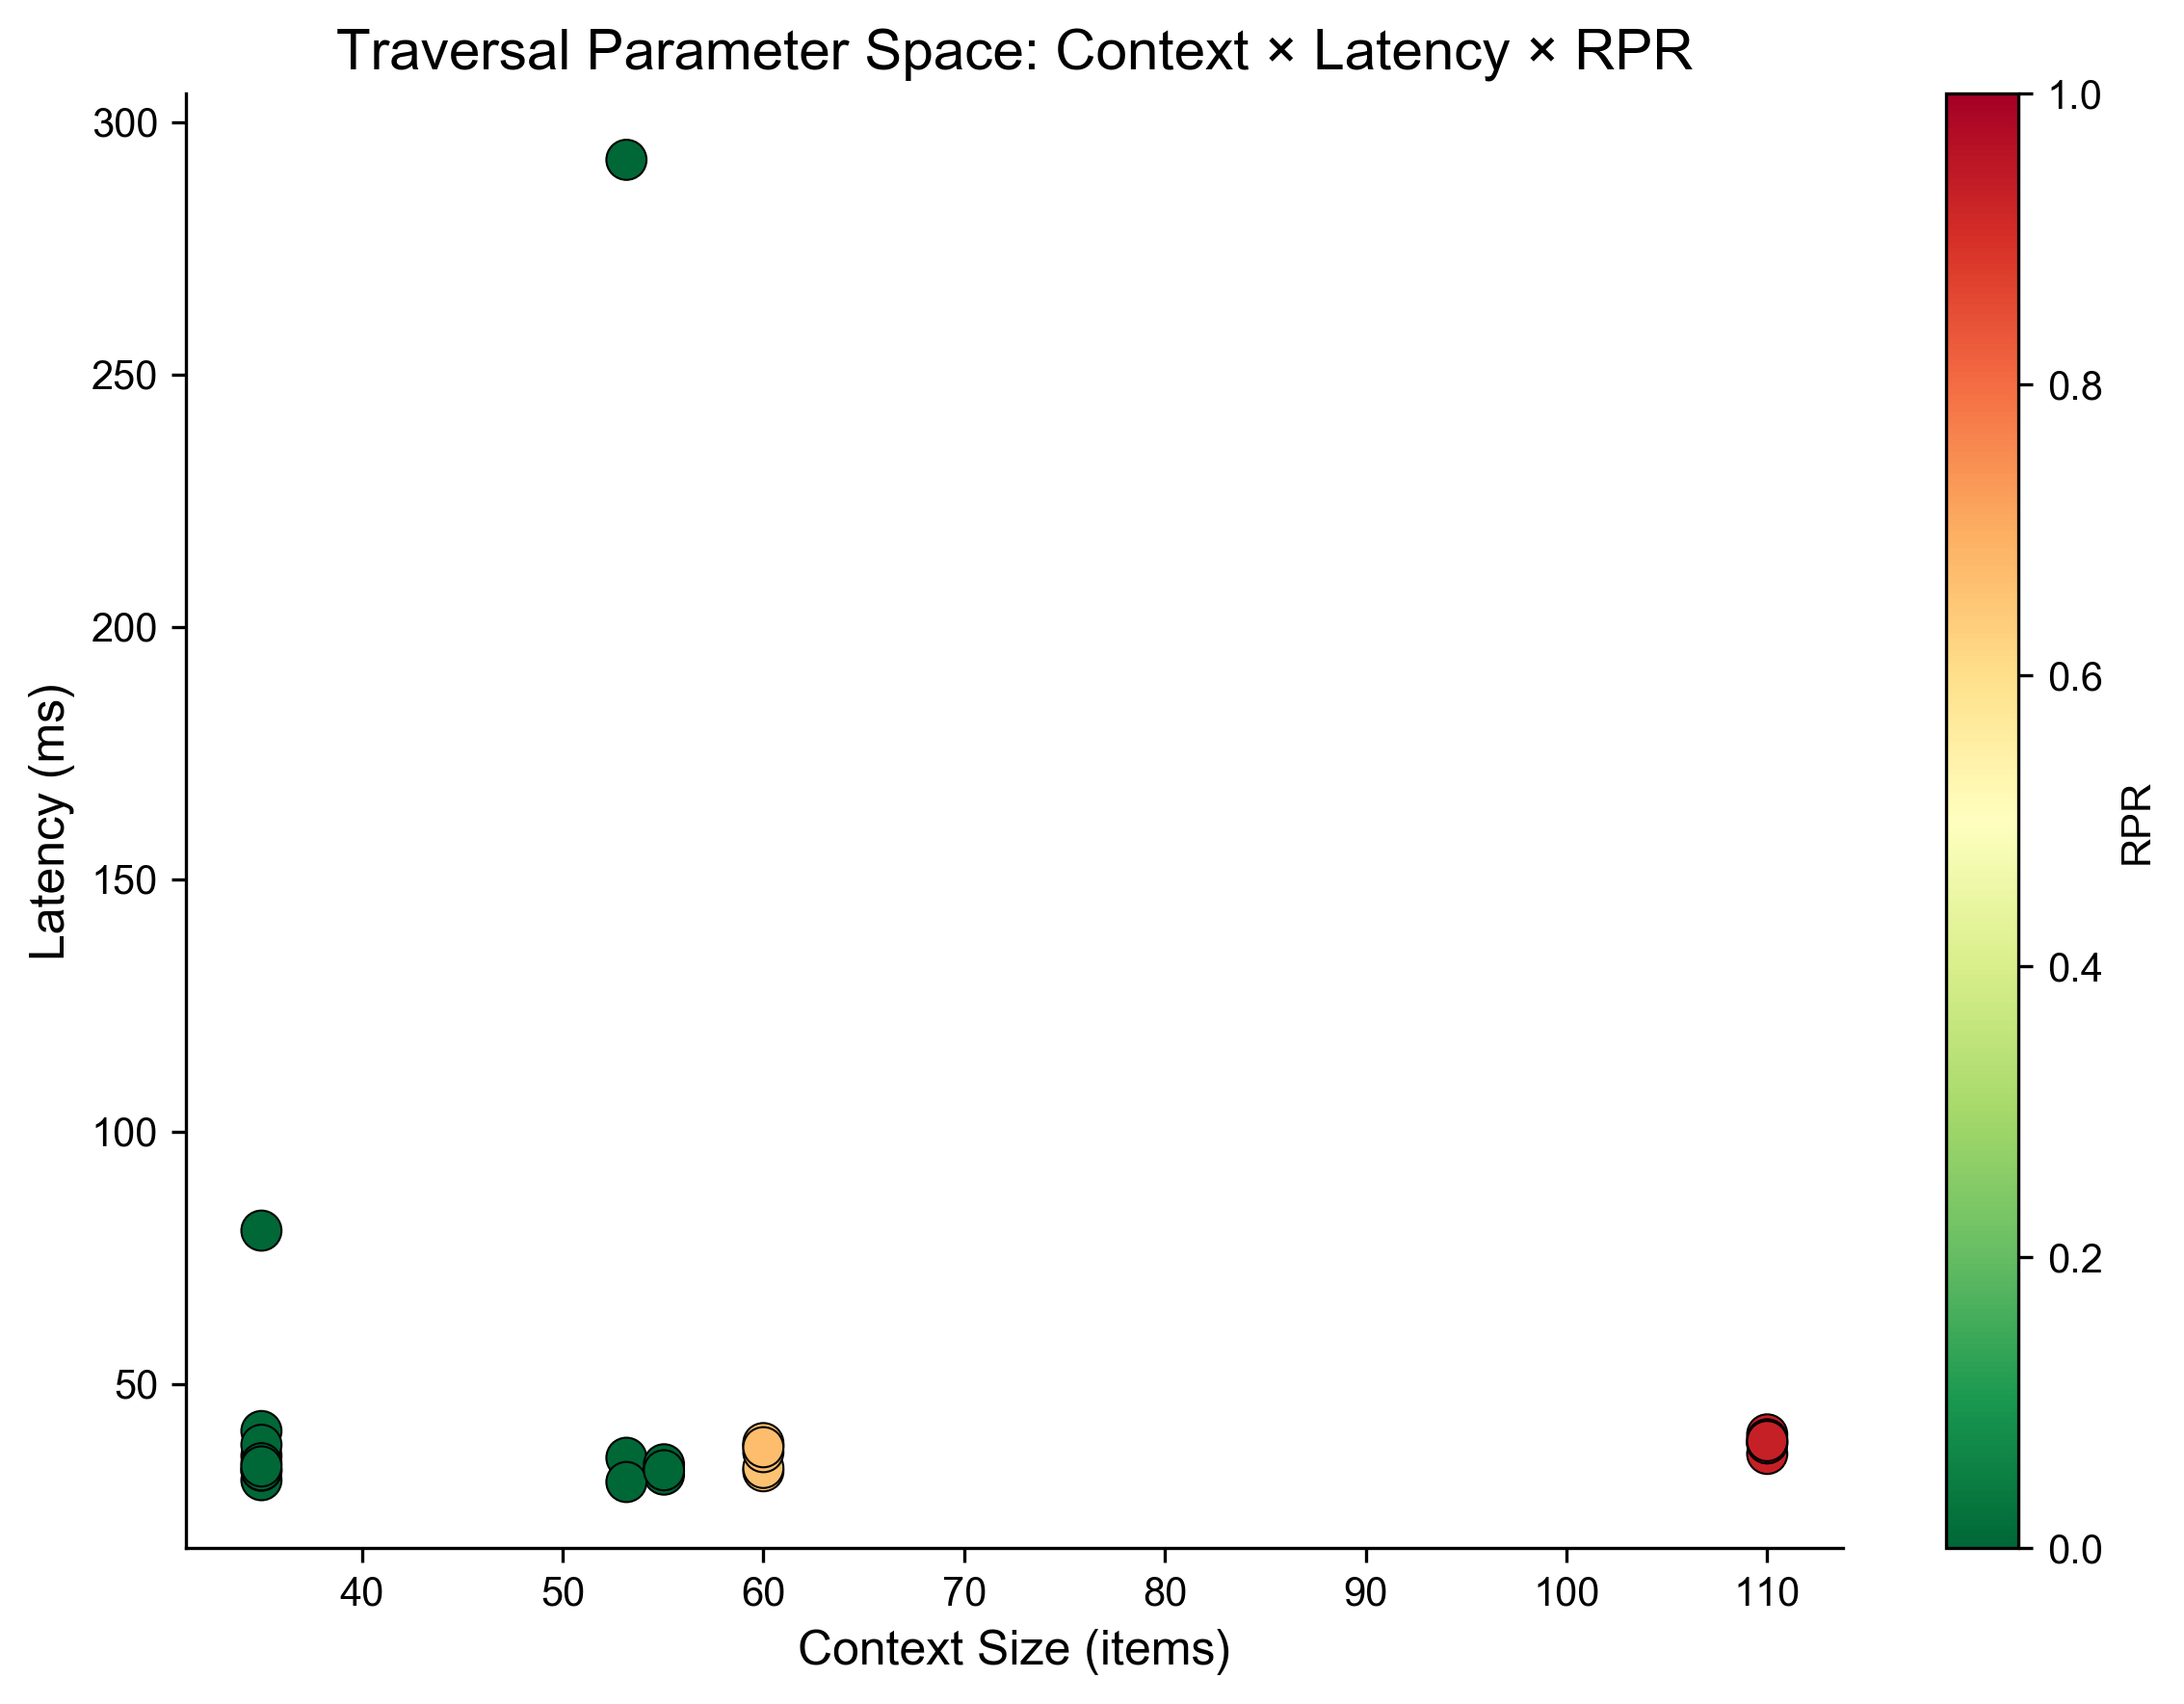
\includegraphics[width=\columnwidth]{figures/traversal_pareto.png}
\caption{Traversal parameter sweep: context size vs.~latency,
  colored by RPR. The total node budget is the primary
  leakage-controlling parameter.}
\label{fig:traversal}
\end{figure}

Three findings emerge:

\textbf{Total node budget is the primary control.} Regardless of
depth or branching, $\text{total\_nodes} = 25$ yields $\text{RPR} = 0$
(insufficient expansion to reach cross-tenant content),
$\text{total\_nodes} = 50$ yields $\text{RPR} \approx 0.66$, and
$\text{total\_nodes} = 100$ yields $\text{RPR} \approx 0.93$. This
is because the total node budget caps how many graph nodes are
gathered, and once this cap prevents expansion from reaching the 2-hop
cross-tenant chunks, leakage is eliminated.

\textbf{Depth must be $\geq 2$ for leakage to occur.} At
$\text{depth} = 1$, $\text{RPR} = 0$ regardless of branching or
total node budget, because single-hop expansion cannot cross the
chunk$\to$entity$\to$chunk pivot path. This confirms the structural
PD=2 signature.

\textbf{Branching factor is irrelevant given a total node cap.} At
fixed depth and total node budget, branching $\in \{5, 10, 25\}$
produces identical RPR values. The BFS expansion fills the node budget
regardless of how many children are explored per node.

\subsection{Latency and Overhead}

Table~\ref{tab:latency} presents latency and context size across
pipeline variants.

\begin{table}[t]
\centering
\caption{Latency (ms) and context size across pipeline variants.}
\label{tab:latency}
\small
\begin{tabular}{l|ccc|c}
\toprule
\textbf{Variant} & \textbf{p50} & \textbf{p95} & \textbf{Mean} &
  \textbf{Ctx} \\
\midrule
\multicolumn{5}{c}{\textit{Benign Queries}} \\
\midrule
  P1 (Vector) & 12.6 & 19.9 & 16.2 & 10 \\
  P3 (Hybrid) & 26.7 & 38.1 & 32.4 & 110 \\
  P4 (+D1) & 26.5 & 34.4 & 30.4 & 56 \\
  P6 (+D1--D3) & 23.1 & 29.8 & 26.4 & 29 \\
  P8 (All) & 22.7 & 28.6 & 25.6 & 20 \\
\midrule
\multicolumn{5}{c}{\textit{Adversarial Queries}} \\
\midrule
  P1 (Vector) & 12.3 & 34.6 & 23.5 & 10 \\
  P3 (Hybrid) & 27.3 & 40.2 & 33.7 & 110 \\
  P4 (+D1) & 26.3 & 32.2 & 29.3 & 50 \\
  P6 (+D1--D3) & 23.1 & 33.7 & 28.4 & 28 \\
  P8 (All) & 22.9 & 30.1 & 26.5 & 20 \\
\bottomrule
\end{tabular}
\end{table}

D1 adds negligible latency overhead---P3 to P4 shows $<$1ms increase
at p50 (26.7$\to$26.5ms benign). More striking, the full defense
stack (P8) is actually \emph{faster} than undefended P3 (22.7 vs.
26.7ms) because budgeted traversal (D3) and trust filtering (D4)
reduce the number of nodes expanded and processed, decreasing both
graph query time and context assembly overhead.

\subsection{Metadata Integrity Stress Test}
\label{sec:mislabel}

An adaptive attacker might attempt to circumvent D1 by corrupting
sensitivity labels. We test D1's robustness by randomly flipping
sensitivity labels on $r\%$ of graph nodes
($r \in \{0.1, 0.5, 1.0, 2.0, 5.0\}$) and measuring RPR under
P4. Results: \textbf{D1 maintains $\text{RPR} = 0.0$ at all
mislabel rates up to 5\%.} This robustness arises because D1's
primary protection is the \emph{tenant} filter (not the sensitivity
filter): cross-tenant leakage requires traversing to a node with a
different tenant label, and sensitivity mislabeling does not affect
tenant assignments. We note that context size decreases slightly at
higher mislabel rates (56$\to$48 items at 5\%) as some authorized
nodes have their sensitivity erroneously raised above the user's
clearance.

\begin{figure}[t]
\centering
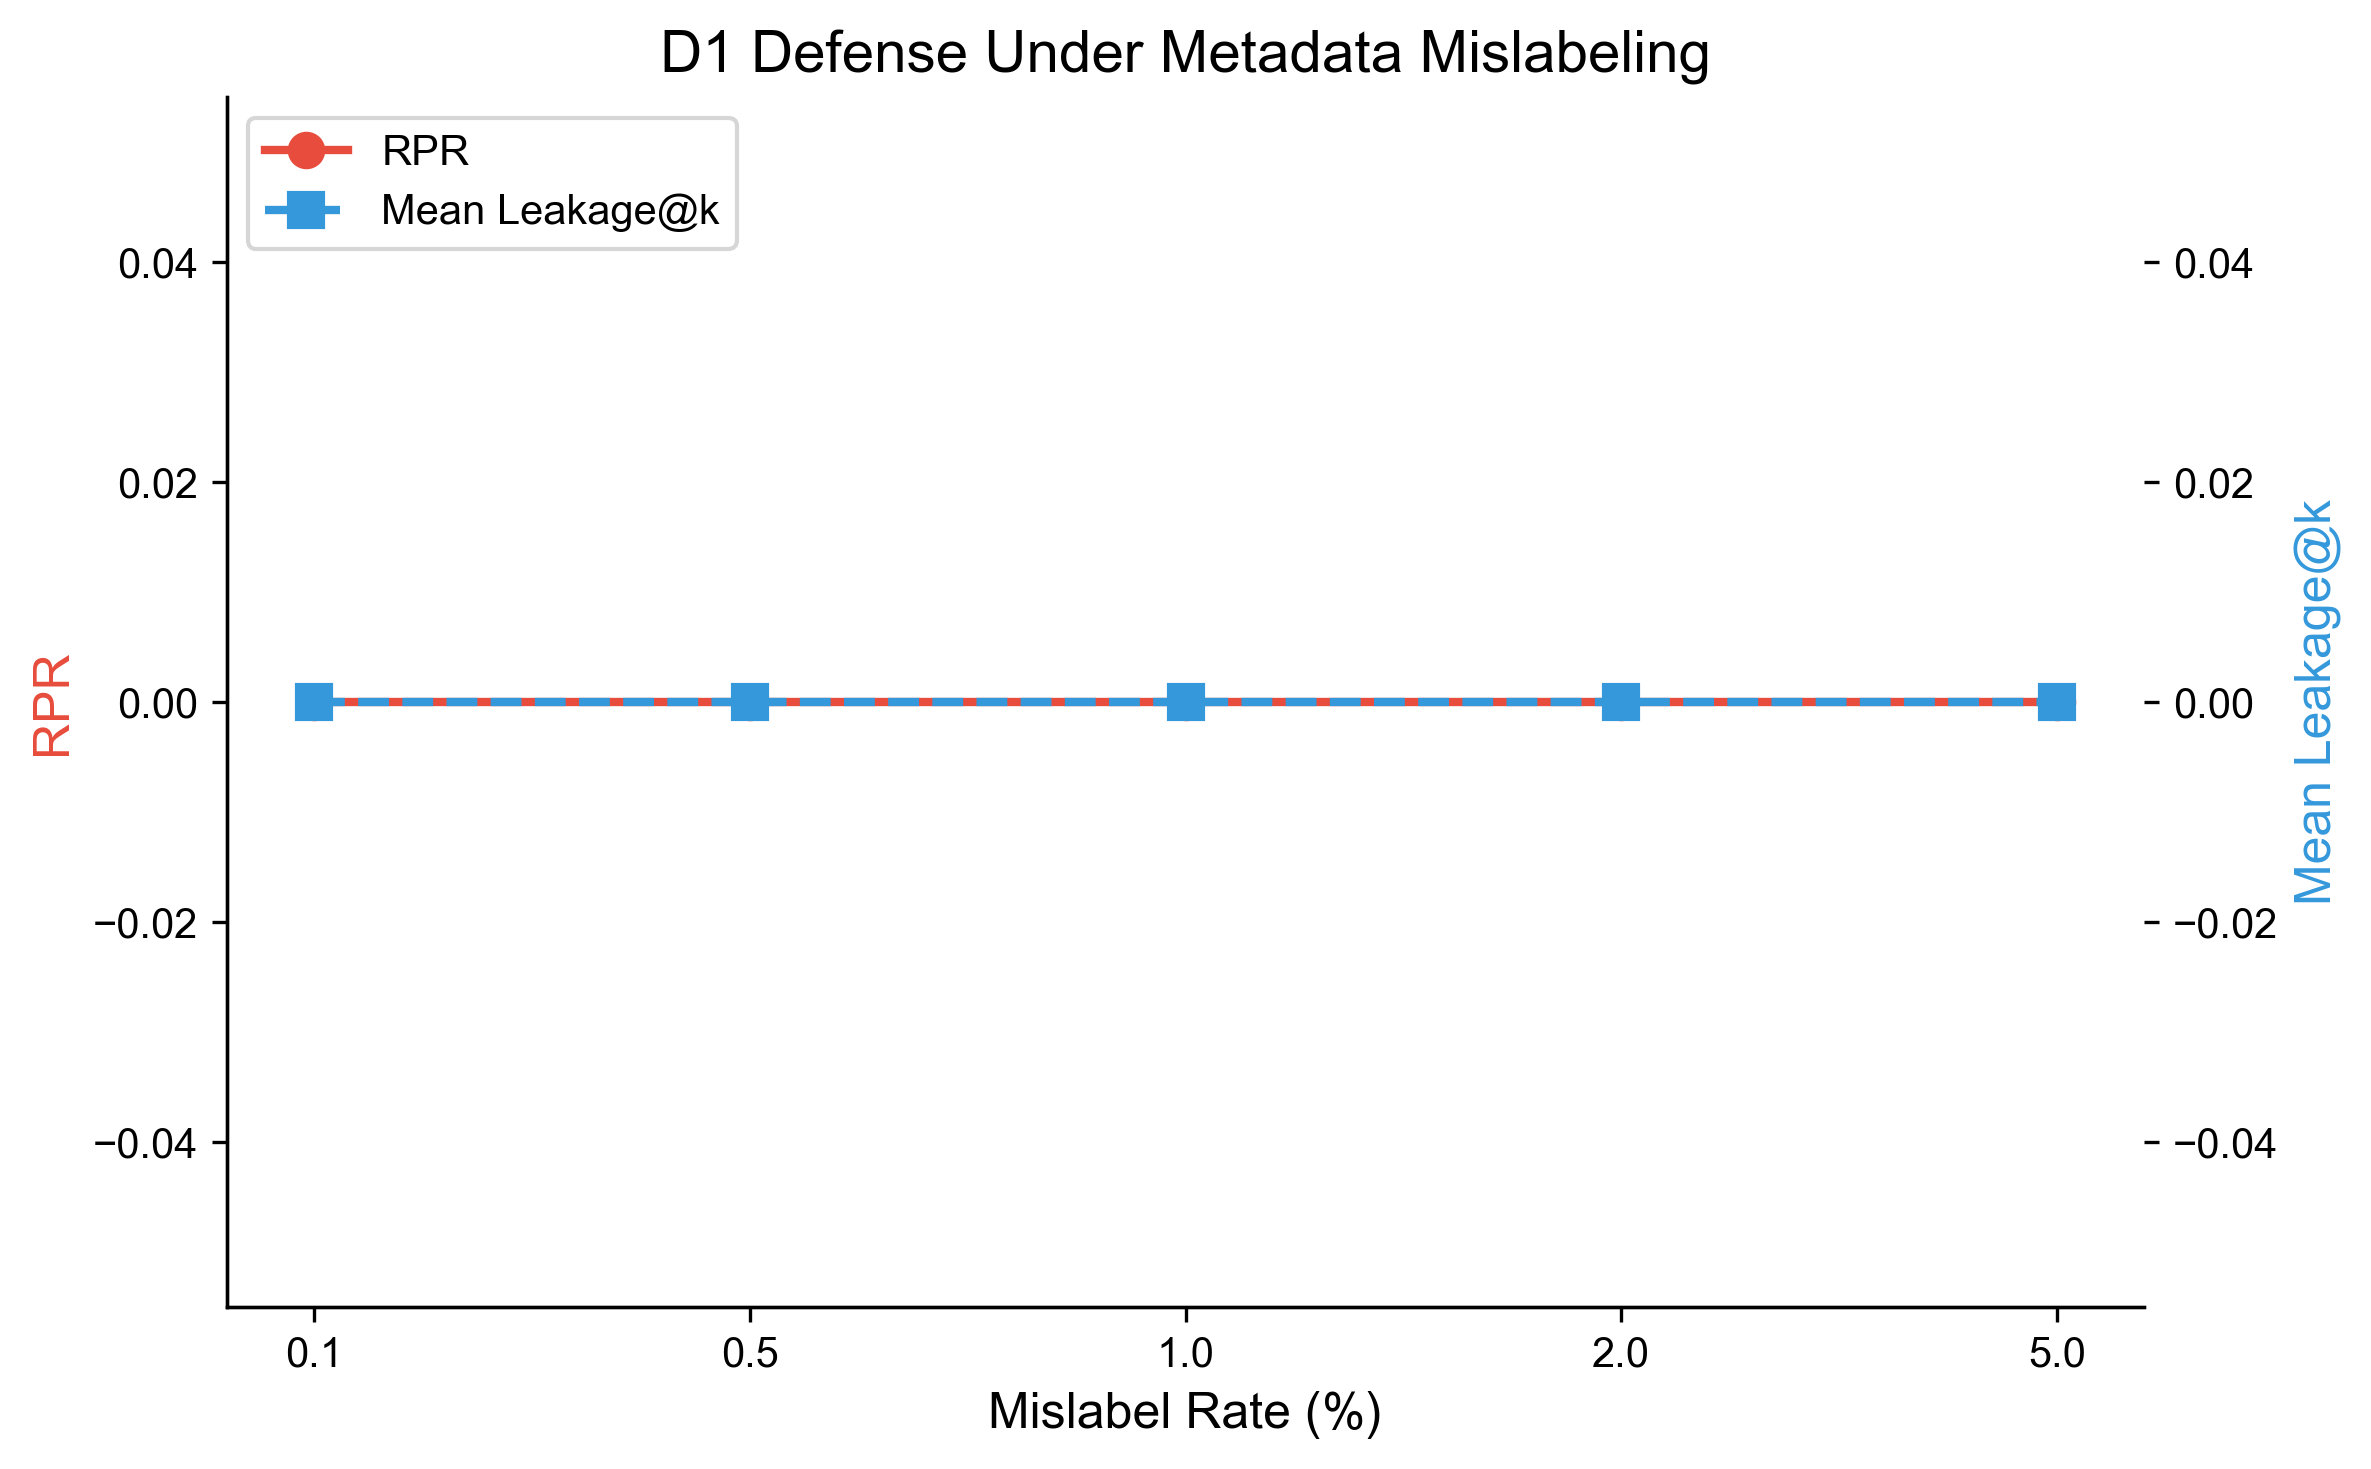
\includegraphics[width=\columnwidth]{figures/mislabel_rate.png}
\caption{D1 robustness under metadata corruption. RPR remains 0.0
  even at 5\% mislabel rate. Context size decreases slightly as
  erroneously up-labeled nodes are filtered.}
\label{fig:mislabel}
\end{figure}

\subsection{Defense Ablation}
\label{sec:defense-ablation}

The defense stack shows a clear pattern
(Figure~\ref{fig:context}):

\begin{itemize}
\item \textbf{D1 alone} (P4): RPR drops from $0.95$ to $0.0$.
  Context reduces from 110 to 50--56 items (the unauthorized items
  are removed; authorized graph-expanded content is retained).
\item \textbf{D1 + D2} (P5): No additional security improvement;
  context remains similar (51--57). Edge allowlisting provides defense
  in depth but does not further reduce leakage already eliminated
  by D1.
\item \textbf{D1--D3} (P6): Context drops to 28--29. Budgeted
  traversal caps the number of expanded nodes, reducing context noise
  from authorized but irrelevant graph content.
\item \textbf{D1--D4} (P7): Context drops to 24--28.
  Trust-weighted filtering removes low-provenance nodes.
\item \textbf{D1--D5} (P8): Context reaches 19--20 items. The merge
  filter provides a final defense-in-depth check, reducing context
  by 82\% from the undefended baseline.
\end{itemize}

\begin{figure}[t]
\centering
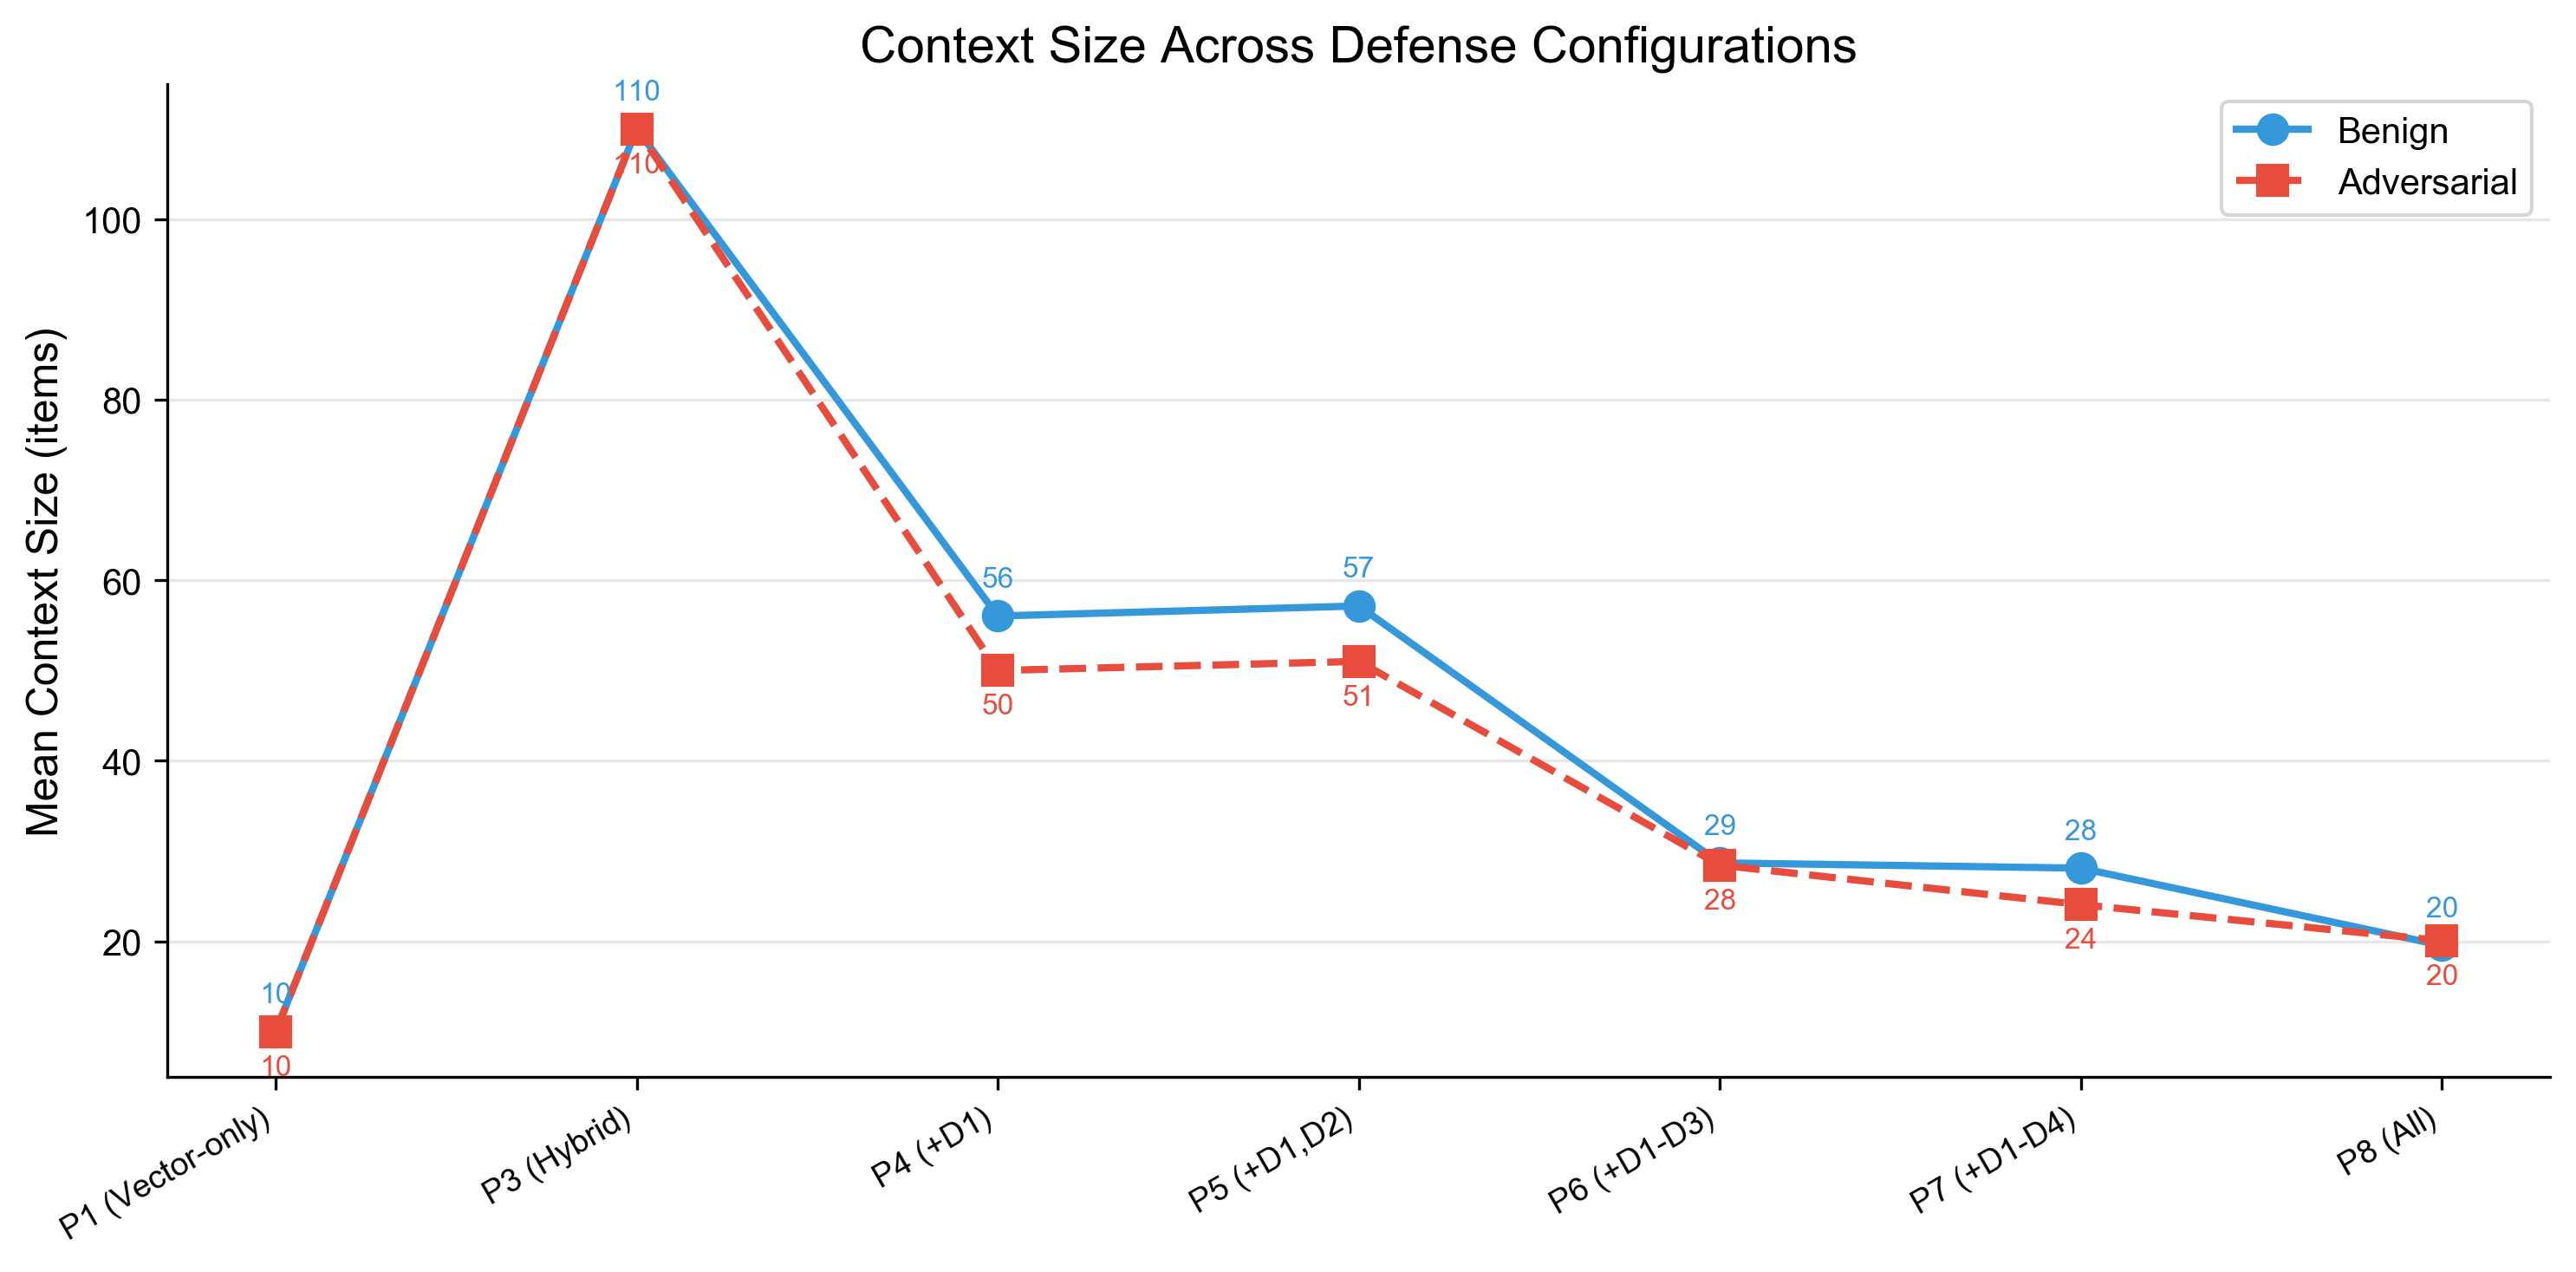
\includegraphics[width=\columnwidth]{figures/context_size.png}
\caption{Mean context size under progressive defenses. D1 alone
  reduces context from 110 to 50--56 items (removing unauthorized
  content). D3--D5 further reduce noise, reaching 19--20 items with
  the full defense stack.}
\label{fig:context}
\end{figure}

The key insight is that D1 is both \emph{necessary and sufficient}
for security (eliminating all leakage), while D2--D5 serve as
\emph{utility optimizers} (reducing context noise and providing
defense in depth).

% ============================================================
\section{Mitigations}
\label{sec:mitigations}

We propose five defenses that operate at different stages of the
hybrid pipeline, forming a defense-in-depth architecture
(Table~\ref{tab:defenses}).

\begin{table}[t]
\centering
\caption{Defense mechanisms, pipeline integration points, and
  experimental impact.}
\label{tab:defenses}
\small
\begin{tabular}{l|l|l}
\toprule
\textbf{Defense} & \textbf{Stage} & \textbf{Effect} \\
\midrule
D1: Per-hop authz & Post-expansion & RPR $\to$ 0.0 \\
D2: Edge allowlist & Traversal query & Defense in depth \\
D3: Budget & Traversal params & Ctx 110 $\to$ 28 \\
D4: Trust weight & Post-expansion & Low-prov removal \\
D5: Merge filter & Post-merge & Final backstop \\
\bottomrule
\end{tabular}
\end{table}

\subsection{D1: Per-Hop Authorization}

Per-hop authorization re-checks access control predicates on every
node reached during graph expansion. For each expanded node $v$, the
defense evaluates:

\begin{equation}
\text{auth}(u, v) = (v.\text{tenant} = t_u) \wedge
  (v.\text{sensitivity} \leq \ell_u)
\end{equation}

Nodes failing this check are removed from the expansion result before
context assembly. In our implementation, D1 operates as a
\textbf{post-expansion filter}: the BFS traversal runs
unrestricted, and the authorization check is applied to the result
set. This is simpler to implement than in-traversal pruning
(which would stop expansion at unauthorized nodes) but is less
efficient because it expands nodes that will be discarded. A true
per-hop pruning implementation would stop expansion at unauthorized
nodes, preventing their children from being explored. We chose
post-expansion filtering for implementation simplicity; the security
properties are identical (both produce $\text{RPR} = 0.0$), but
in-traversal pruning would further reduce latency and context
processing overhead.

D1 is the most effective defense: it reduces RPR from 0.95 to 0.0
across all query types and all attack variants, with $<$1ms latency
overhead.

The critical insight is that \emph{existing graph databases already
store the metadata needed for this check} (tenant labels, sensitivity
tiers). The defense does not require new infrastructure---only the
discipline to re-check authorization at the graph layer rather than
relying solely on the vector prefilter.

\subsection{D1 Metadata Integrity Assumption}
\label{sec:metadata-integrity}

D1 assumes that node metadata (tenant, sensitivity) is trustworthy.
If an attacker can forge metadata during document injection, D1 can
be bypassed. Our metadata stress test (\S\ref{sec:mislabel}) shows
that D1 is robust to random mislabeling up to 5\%, but targeted
metadata forgery is a different threat. Mitigations include:
(a) system-assigned metadata during ingestion (the uploader cannot
choose tenant or sensitivity labels), (b) cryptographic signing of
metadata at ingestion time, and (c) periodic metadata audits that
compare node labels against source-of-truth identity systems. In
practice, most enterprise document management systems already enforce
system-assigned tenant labels, making (a) the natural deployment
model.

\subsection{D2: Edge Allowlist}

Edge allowlisting restricts graph traversal to pre-approved edge
types per query class. The expander's BFS query includes a
\texttt{relationshipFilter} parameter that limits which edge types
can be traversed. For example, general queries may traverse MENTIONS,
DEPENDS\_ON, and BELONGS\_TO edges, while RELATED\_TO edges (which
are the primary vector for bridge attacks) are excluded.

\subsection{D3: Budgeted Traversal}

Budgeted traversal enforces hard limits on BFS expansion: maximum hop
depth, maximum branching factor per node, and maximum total expanded
nodes. Our traversal sweep (\S\ref{sec:traversal-sweep}) shows that
$\text{total\_nodes} \leq 25$ eliminates leakage even without D1,
while the default budget ($d_\text{max}=2$, branching $\leq 10$,
total $\leq 50$) reduces context from 56 items (D1 only) to 28 items,
removing authorized but irrelevant graph content that adds noise.

\subsection{D4: Trust-Weighted Expansion}

Trust-weighted expansion filters expanded nodes by their provenance
score. Each node carries a provenance score ($0.0$--$1.0$) based on
its source reliability. The defense applies a minimum threshold
(default: 0.6), removing low-provenance content. This is particularly
effective against injected attack payloads, which carry provenance
scores of 0.3--0.4 in our attack implementations.

\subsection{D5: Merge-Time Policy Filter}

The merge-time policy filter performs a final access control check
after vector and graph results are combined. This defense acts as a
backstop: even if earlier defenses miss an unauthorized item, the
merge filter removes any item whose sensitivity exceeds the user's
clearance before the context reaches the LLM.

% ============================================================
\section{Discussion}
\label{sec:discussion}

\subsection{Security-Utility Tradeoff}

Our results reveal a favorable security-utility tradeoff. D1 alone
achieves complete security ($\text{RPR} = 0.0$) while retaining 50\%
of the graph-expanded context ($110 \to 50\text{--}56$ items). The
retained items are authorized content that contributes to answer
quality. Adding D3--D5 further reduces context to 19--20
items---an 82\% reduction from the undefended baseline---but the
additional defenses trade context volume for noise reduction rather
than security improvement.

The practical recommendation is clear: \textbf{deploy D1 immediately
as a minimum viable defense.} Add D3 and D4 if context noise is
impacting LLM generation quality. D2 and D5 provide defense in
depth for compliance-sensitive deployments.

\subsection{Why PD = 2 in Our Construction}

The uniform $\text{PD} = 2$ finding reflects a structural property
of hybrid RAG systems that construct a bipartite graph between chunks
and entities. The entity-linking step inherently creates a 2-hop
path between any two chunks that mention the same entity: Chunk A
(hop 0) $\to$ shared entity (hop 1) $\to$ Chunk B (hop 2). This
means that \emph{every shared entity is a potential pivot}, and
the number of pivot opportunities scales with the number of
cross-boundary entity mentions.

In our corpus, 40 entities are naturally shared across tenant
boundaries---not through adversarial injection, but through
legitimate organizational references. Shared infrastructure
(``auth-service''), shared vendors (``CloudCorp''), and shared
compliance standards (``SOC2-audit'') create organic cross-tenant
entity mentions that the entity linker faithfully connects.

Knowledge graphs with richer topologies---ontological hierarchies,
multi-hop inference chains, entity-to-entity relationships beyond
simple co-mention---may exhibit leakage at PD $> 2$. Our traversal
sweep confirms that depth=1 prevents all leakage in the bipartite
construction, but graphs with entity-entity edges would require
analysis at deeper traversal depths.

\subsection{The Amplification Mechanics}

The core insight of this work is not simply ``apply ACLs to graph
expansion'' but rather the \emph{identification and characterization
of a compound attack surface} that arises from combining two
individually secure retrieval modalities. Vector retrieval with
tenant prefiltering is secure ($\text{RPR} = 0.0$). Graph retrieval
within a single tenant's subgraph is secure. But connecting
vector retrieval outputs to graph expansion inputs---the pivot
boundary---creates leakage that neither modality exhibits alone.

This is analogous to composition vulnerabilities in other
security domains: two individually secure components can produce
an insecure system when composed. The amplification factor
($\text{AF}(\epsilon) \approx 160\text{--}194\times$) quantifies
the severity: hybrid RAG does not incrementally increase leakage---it
creates $160\times$ more leaked items than the vector baseline from
which it amplifies.

The defense implication is equally specific: the authorization
check must be placed \emph{at the boundary}, after graph expansion
and before context assembly. Authorization at the vector layer
alone (which every production system already has) is insufficient.
Authorization at the LLM layer (e.g., instruction-following) is
unreliable. Only authorization at the graph expansion layer---the
pivot boundary itself---addresses the root cause.

\subsection{Comparison with Prior Art}

GRAGPoison~\cite{gragpoison2026} demonstrates that graph structure
amplifies small poisoning inputs (98\% ASR from relation injection).
Our work extends this insight to hybrid architectures: the
\emph{combination} of vector retrieval and graph expansion creates a
compound attack surface where authorized vector results seed
unauthorized graph traversals.

PoisonedRAG~\cite{zou2025poisonedrag} achieves 90\% ASR by injecting
5 documents into vector stores. In vector-only RAG, this is
contained by prefilters. In hybrid RAG, even a single retrieved
document that mentions a shared entity can trigger graph expansion
into sensitive neighborhoods, making the effective attack surface
orders of magnitude larger.

The Graph RAG Privacy Paradox~\cite{graphragprivacy2025} observes
that graph RAG reduces text leakage but increases structural
information extraction. Our findings align: the hybrid pipeline's
graph expansion systematically transforms authorized text into
unauthorized structural access.

\subsection{Implications for Agentic Systems}

The pivot attack is especially dangerous in agentic RAG deployments
(LangGraph, CrewAI) where graph traversal is performed autonomously
by an LLM agent~\cite{multiagentic2025}. In these systems, the
agent decides traversal depth, edge types, and expansion strategies
without human oversight. A poisoned vector seed can manipulate the
agent into performing unrestricted graph exploration, and research
shows that a single compromised agent can poison 87\% of downstream
decision-making within 4 hours~\cite{multiagentic2025}. Per-hop
authorization is even more critical in agentic settings, where there
is no human in the loop at the expansion step.

% ============================================================
\section{Limitations}
\label{sec:limitations}

\textbf{Synthetic dataset.} Our corpus is synthetically generated,
not drawn from production enterprise data. While the entity
distributions, tenant structures, and sensitivity tiers are designed
to mirror realistic deployments, real-world knowledge graphs may
exhibit different connectivity patterns that affect pivot attack
reach. The bipartite chunk-entity graph topology in our construction
produces a uniform PD=2 signature that may not hold in graphs with
richer entity-to-entity relationships.

\textbf{Retrieval-only measurement.} We measure what enters the LLM's
context window but do not evaluate whether the LLM reproduces
sensitive content in its generation. An LLM might ignore unauthorized
context items, reducing the practical impact of measured leakage.
Conversely, chain-of-thought reasoning might amplify the impact by
synthesizing cross-tenant connections.

\textbf{Two embedding models.} We evaluate two open-source models
(all-MiniLM-L6-v2, 384d, and all-mpnet-base-v2, 768d) and confirm
the vulnerability persists across both (\S\ref{sec:embedding}).
However, we do not test commercial embedding models (e.g., OpenAI
text-embedding-3-large) which may produce different similarity
distributions. The pivot vulnerability is structural (entity linking,
not embedding quality), so we expect model independence to hold broadly.

\textbf{Non-adaptive attacker.} Our attacks are crafted against the
baseline pipeline. While we evaluate adaptive strategies against D1
(metadata corruption, \S\ref{sec:mislabel}) and show robustness up to
5\% mislabel rates, we do not evaluate attackers who target D2--D5
specifically (e.g., crafting high-provenance payloads to bypass D4).

\textbf{Graph-only baseline (P2).} We omit a graph-only RAG baseline
because graph-only retrieval without vector seeding does not involve
the pivot boundary under study. This means our results characterize
the \emph{hybrid-specific} vulnerability but do not compare against
graph-only retrieval's independent security properties.

% ============================================================
\section{Related Work}
\label{sec:related_work}

\subsection{Vector RAG Poisoning}

PoisonedRAG~\cite{zou2025poisonedrag} formalized knowledge corruption
attacks on RAG, achieving 90\% ASR with 5 injected documents.
CorruptRAG~\cite{corruptrag2025} demonstrated single-document attacks
with higher stealth. CtrlRAG~\cite{ctrlrag2025} achieved 90\% ASR on
GPT-4o via black-box feedback optimization.
RIPRAG~\cite{riprag2025} applied reinforcement learning to optimize
poisoning without model access.
NeuroGenPoisoning~\cite{neurogenpoison2025} targeted specific neurons
for >90\% success. These works study vector-side attacks in isolation;
none address what happens when poisoned vector results seed graph
expansion.

\subsection{GraphRAG Security}

GRAGPoison~\cite{gragpoison2026} is the closest related work,
demonstrating relation-centric poisoning of GraphRAG with 98\% ASR.
TKPA~\cite{fewwords2025} showed that modifying 0.06\% of corpus text
drops GraphRAG accuracy by 45 percentage points.
RAGCrawler~\cite{ragcrawler2026} achieved 84.4\% knowledge extraction
coverage through graph-guided probing. The Graph RAG Privacy
Paradox~\cite{graphragprivacy2025} established that graph RAG
increases structural leakage while reducing text leakage. Our work
extends these graph-side insights to the hybrid setting, where the
vector-to-graph transition creates a compound attack surface.

\subsection{RAG Privacy and Extraction}

The SoK on RAG Privacy~\cite{sokprivacy2026} systematized all known
privacy attack vectors in RAG systems and explicitly noted that hybrid
RAG privacy risks remain under-studied. Riddle Me
This~\cite{riddleme2025} demonstrated membership inference on RAG
systems. Traceback of RAG
Poisoning~\cite{traceback2025} provided forensic methods for
identifying responsible documents, but traces only through the vector
retrieval path without following graph expansion chains.

\subsection{RAG Defenses}

RAGuard~\cite{raguard2025} detects poisoning via retrieval pattern
analysis. SeCon-RAG~\cite{seconrag2025} applies semantic consistency
filtering. RevPRAG~\cite{revprag2025} achieves 98\% detection via
LLM activation analysis. SDAG~\cite{sdag2026} partitions context
into trusted and untrusted segments with block-sparse attention.
SD-RAG~\cite{sdrag2026} implements selective disclosure policies.
All operate within a single retrieval modality. Our defense suite
(D1--D5) is the first designed specifically for the cross-store
boundary, with per-hop authorization as the cornerstone mechanism.

% ============================================================
\section{Conclusion}
\label{sec:conclusion}

Hybrid RAG pipelines that combine vector retrieval with knowledge
graph expansion introduce a previously unstudied attack surface at
the vector-to-graph boundary. We formalized this threat as Retrieval
Pivot Risk (RPR) and demonstrated through 500 evaluation queries with
bootstrap confidence intervals that undefended hybrid pipelines
exhibit $\text{RPR} = 0.95 \pm 0.02$---compared to $0.0$ for
vector-only retrieval---with all leakage occurring at 2 hops through
the entity-linking pivot in our bipartite graph construction.

Our taxonomy of four Retrieval Pivot Attacks shows that small
injection budgets (10--20 chunks) can exploit this boundary through
seed steering, entity anchoring, neighborhood flooding, and bridge
node creation. More significantly, we showed that even without
adversarial injection, the 40 naturally shared entities in our
multi-tenant knowledge graph create organic pivot paths that leak
cross-tenant data at $\text{RPR} = 0.954$.

The most important finding is practical: \textbf{per-hop
authorization---re-checking tenant and sensitivity labels at each
graph expansion step---eliminates all measured retrieval pivot
leakage across 500 queries, all four attack variants, and metadata
mislabel rates up to 5\%.} This defense is simple, requires no model
changes, adds $<$1ms latency, and uses metadata already present in
graph databases. We recommend it as the minimum viable security
control for any hybrid RAG deployment.

Our traversal parameter sweep reveals that the total node budget is
the primary leakage-controlling parameter: limiting expansion to
$\leq$25 nodes eliminates leakage even without authorization checks,
while expansion depth must reach $\geq$2 for the pivot to occur. The
full defense stack (D1--D5) reduces context noise by 82\% with zero
residual leakage.

Our connectivity sweep (\S\ref{sec:connectivity}) shows that even zero
intentional bridge entities produce $\text{RPR} = 0.93$ through
organic NER overlap, while our embedding model comparison
(\S\ref{sec:embedding}) confirms that higher-quality embeddings
slightly \emph{increase} leakage rather than mitigate it. These
findings reinforce the structural nature of the vulnerability.

Our work opens several directions for future research: evaluation on
production enterprise graphs with richer entity-to-entity topologies
(where PD $>$ 2 may emerge), adaptive attacker strategies that target
metadata integrity or craft high-provenance payloads to bypass D4,
LLM generation-level impact measurement (does the LLM actually
reproduce leaked content?), and extension to agentic hybrid RAG where
graph traversal is autonomously controlled.

% ============================================================
\bibliographystyle{IEEEtran}
\bibliography{references}

% ============================================================
\appendix
\section{Artifact Appendix}
\label{sec:artifact}

\subsection{Repository}

The complete codebase, synthetic data generators, attack
implementations, defense suite, evaluation harness, and experimental
results are available at:
\url{https://github.com/scthornton/hybrid-rag-pivot-attacks}

\subsection{System Requirements}

\begin{itemize}
\item Python 3.11+ with dependencies: \texttt{chromadb},
  \texttt{neo4j}, \texttt{spacy}, \texttt{sentence-transformers},
  \texttt{pydantic}, \texttt{numpy}
\item Neo4j 5.15+ with APOC plugin (for
  \texttt{apoc.path.spanningTree})
\item ChromaDB server (latest)
\item spaCy model: \texttt{en\_core\_web\_sm}
\end{itemize}

\subsection{Reproduction Steps}

\begin{enumerate}
\item Clone repository and install: \texttt{pip install -e ".[dev]"}
\item Start services: \texttt{docker compose up -d} (Neo4j + ChromaDB)
\item Generate corpus: \texttt{python scripts/make\_synth\_data.py}
\item Generate queries: \texttt{python scripts/generate\_queries.py}
\item Build indexes: \texttt{python scripts/build\_indexes.py}
\item Run experiments: \texttt{python scripts/run\_experiments.py
  --bootstrap}
\item Run attack experiments: \texttt{python
  scripts/run\_attack\_experiments.py}
\item Run sweeps: \texttt{python scripts/run\_sweep\_experiments.py
  --traversal-sweep --mislabel-sweep --connectivity-sweep}
\item Run embedding sensitivity: \texttt{python
  scripts/build\_indexes.py --embed-model all-mpnet-base-v2
  --chroma-collection pivorag\_chunks\_mpnet} then
  \texttt{python scripts/run\_experiments.py --embed-model
  all-mpnet-base-v2 --chroma-collection pivorag\_chunks\_mpnet}
\item Analyze organic leakage: \texttt{python
  scripts/analyze\_organic\_leakage.py}
\item Export results: \texttt{python scripts/export\_results.py
  --latest}
\item Run tests: \texttt{pytest tests/ -v} (78 tests passing)
\end{enumerate}

\balance
\end{document}
